\IfFileExists{stacks-project.cls}{%
\documentclass{stacks-project}
}{%
\documentclass{amsart}
}
\usepackage{amssymb}

% For dealing with references we use the comment environment
\usepackage{verbatim}
\newenvironment{reference}{\comment}{\endcomment}
%\newenvironment{reference}{}{}
\newenvironment{slogan}{\comment}{\endcomment}
\newenvironment{history}{\comment}{\endcomment}

% For commutative diagrams we use Xy-pic
\usepackage[all]{xy}

% We use 2cell for 2-commutative diagrams.
\xyoption{2cell}
\UseAllTwocells

% We use multicol for the list of chapters between chapters
\usepackage{multicol}

% This is generally recommended for better output
\usepackage{lmodern}
\usepackage[T1]{fontenc}
\usepackage{textalpha}

% For cross-file-references
% We prefer the snapshot tmp/xref/#2.aux,
% which latexmkrc replaces atomically, so
% that documents compiled simultaneously
% never read a half-written .aux file.
% The last argument keeps links to #2.pdf.
\usepackage{xr-hyper}
\newcommand{\maybeexternaldocument}[2]{%
  \IfFileExists{#2.aux}{%
    \externaldocument[#1]{#2}%
  }{%
    \PackageWarning{stack}{Missing #2.aux; external references with prefix #1 unavailable}%
  }%
}
\let\externaldocumentorig\externaldocument
\renewcommand{\externaldocument}[2][]{%
  \IfFileExists{tmp/xref/#2.aux}{%
    \externaldocumentorig[#1]{tmp/xref/#2}[#2.pdf]%
  }{%
  \IfFileExists{#2.aux}{%
    \externaldocumentorig[#1]{#2}%
  }{%
    \PackageWarning{stack}{Missing #2.aux; external references with prefix #1 unavailable}%
  }%
  }%
}

% Package for hypertext links:
\usepackage{hyperref}

% For any local file, say "hello.tex" you want to link to please
% use \externaldocument[hello-]{hello}
\externaldocument[introduction-]{introduction}
\externaldocument[conventions-]{conventions}
\externaldocument[sets-]{sets}
\externaldocument[categories-]{categories}
\externaldocument[topology-]{topology}
\externaldocument[sheaves-]{sheaves}
\externaldocument[sites-]{sites}
\externaldocument[stacks-]{stacks}
\externaldocument[fields-]{fields}
\externaldocument[algebra-]{algebra}
\externaldocument[brauer-]{brauer}
\externaldocument[homology-]{homology}
\externaldocument[derived-]{derived}
\externaldocument[simplicial-]{simplicial}
\externaldocument[more-algebra-]{more-algebra}
\externaldocument[smoothing-]{smoothing}
\externaldocument[modules-]{modules}
\externaldocument[sites-modules-]{sites-modules}
\externaldocument[injectives-]{injectives}
\externaldocument[cohomology-]{cohomology}
\externaldocument[sites-cohomology-]{sites-cohomology}
\externaldocument[dga-]{dga}
\externaldocument[dpa-]{dpa}
\externaldocument[sdga-]{sdga}
\externaldocument[hypercovering-]{hypercovering}
\externaldocument[schemes-]{schemes}
\externaldocument[constructions-]{constructions}
\externaldocument[properties-]{properties}
\externaldocument[morphisms-]{morphisms}
\externaldocument[coherent-]{coherent}
\externaldocument[divisors-]{divisors}
\externaldocument[limits-]{limits}
\externaldocument[varieties-]{varieties}
\externaldocument[topologies-]{topologies}
\externaldocument[descent-]{descent}
\externaldocument[perfect-]{perfect}
\externaldocument[more-morphisms-]{more-morphisms}
\externaldocument[flat-]{flat}
\externaldocument[groupoids-]{groupoids}
\externaldocument[more-groupoids-]{more-groupoids}
\externaldocument[etale-]{etale}
\externaldocument[chow-]{chow}
\externaldocument[intersection-]{intersection}
\externaldocument[pic-]{pic}
\externaldocument[weil-]{weil}
\externaldocument[adequate-]{adequate}
\externaldocument[dualizing-]{dualizing}
\externaldocument[duality-]{duality}
\externaldocument[discriminant-]{discriminant}
\externaldocument[derham-]{derham}
\externaldocument[local-cohomology-]{local-cohomology}
\externaldocument[algebraization-]{algebraization}
\externaldocument[curves-]{curves}
\externaldocument[resolve-]{resolve}
\externaldocument[models-]{models}
\externaldocument[functors-]{functors}
\externaldocument[equiv-]{equiv}
\externaldocument[pione-]{pione}
\externaldocument[etale-cohomology-]{etale-cohomology}
\externaldocument[proetale-]{proetale}
\externaldocument[relative-cycles-]{relative-cycles}
\externaldocument[more-etale-]{more-etale}
\externaldocument[trace-]{trace}
\externaldocument[crystalline-]{crystalline}
\externaldocument[spaces-]{spaces}
\externaldocument[spaces-properties-]{spaces-properties}
\externaldocument[spaces-morphisms-]{spaces-morphisms}
\externaldocument[decent-spaces-]{decent-spaces}
\externaldocument[spaces-cohomology-]{spaces-cohomology}
\externaldocument[spaces-limits-]{spaces-limits}
\externaldocument[spaces-divisors-]{spaces-divisors}
\externaldocument[spaces-over-fields-]{spaces-over-fields}
\externaldocument[spaces-topologies-]{spaces-topologies}
\externaldocument[spaces-descent-]{spaces-descent}
\externaldocument[spaces-perfect-]{spaces-perfect}
\externaldocument[spaces-more-morphisms-]{spaces-more-morphisms}
\externaldocument[spaces-flat-]{spaces-flat}
\externaldocument[spaces-groupoids-]{spaces-groupoids}
\externaldocument[spaces-more-groupoids-]{spaces-more-groupoids}
\externaldocument[bootstrap-]{bootstrap}
\externaldocument[spaces-pushouts-]{spaces-pushouts}
\externaldocument[spaces-chow-]{spaces-chow}
\externaldocument[groupoids-quotients-]{groupoids-quotients}
\externaldocument[spaces-more-cohomology-]{spaces-more-cohomology}
\externaldocument[spaces-simplicial-]{spaces-simplicial}
\externaldocument[spaces-duality-]{spaces-duality}
\externaldocument[formal-spaces-]{formal-spaces}
\externaldocument[restricted-]{restricted}
\externaldocument[spaces-resolve-]{spaces-resolve}
\externaldocument[formal-defos-]{formal-defos}
\externaldocument[defos-]{defos}
\externaldocument[cotangent-]{cotangent}
\externaldocument[examples-defos-]{examples-defos}
\externaldocument[algebraic-]{algebraic}
\externaldocument[examples-stacks-]{examples-stacks}
\externaldocument[stacks-sheaves-]{stacks-sheaves}
\externaldocument[criteria-]{criteria}
\externaldocument[artin-]{artin}
\externaldocument[quot-]{quot}
\externaldocument[stacks-properties-]{stacks-properties}
\externaldocument[stacks-morphisms-]{stacks-morphisms}
\externaldocument[stacks-limits-]{stacks-limits}
\externaldocument[stacks-cohomology-]{stacks-cohomology}
\externaldocument[stacks-perfect-]{stacks-perfect}
\externaldocument[stacks-introduction-]{stacks-introduction}
\externaldocument[stacks-more-morphisms-]{stacks-more-morphisms}
\externaldocument[stacks-geometry-]{stacks-geometry}
\externaldocument[moduli-]{moduli}
\externaldocument[moduli-curves-]{moduli-curves}
\externaldocument[examples-]{examples}
\externaldocument[exercises-]{exercises}
\externaldocument[guide-]{guide}
\externaldocument[desirables-]{desirables}
\externaldocument[coding-]{coding}
\externaldocument[obsolete-]{obsolete}
\externaldocument[fdl-]{fdl}
\externaldocument[index-]{index}

% Heap Project documents
\externaldocument[linear-algebra-]{linear-algebra}
\externaldocument[groups-]{groups}
\externaldocument[complex-analysis-]{complex-analysis}
\externaldocument[functional-analysis-]{functional-analysis}
\externaldocument[categories-]{categories}
\externaldocument[commutative-algebra-]{commutative-algebra}
\externaldocument[ringed-spaces-]{ringed-spaces}
\externaldocument[homological-algebra-]{homological-algebra}
\externaldocument[lie-algebras-]{lie-algebras}
\externaldocument[representation-theory-]{representation-theory}
\externaldocument[smooth-manifolds-]{smooth-manifolds}
\externaldocument[differential-topology-]{differential-topology}
\externaldocument[algebraic-topology-]{algebraic-topology}
\externaldocument[differential-geometry-]{differential-geometry}
\externaldocument[algebraic-geometry-]{algebraic-geometry}
\externaldocument[symplectic-geometry-]{symplectic-geometry}
\externaldocument[complex-geometry-]{complex-geometry}
\externaldocument[hodge-theory-]{hodge-theory}
\maybeexternaldocument{deformations-}{deformations}
\externaldocument[vertex-algebras-]{vertex-algebras}
\externaldocument[springer-]{springer}
\externaldocument[infty-categories-]{infty-categories}
\externaldocument[seminars-differential-geometry-]{%
seminars-differential-geometry}
\externaldocument[seminars-complex-geometry-]{%
seminars-complex-geometry}
\externaldocument[seminars-algebraic-geometry-]{%
seminars-algebraic-geometry}
\externaldocument[seminars-others-]{%
seminars-others}
\externaldocument[%
geometric-prequantization-]{%
geometric-prequantization}
\externaldocument[surfaces-]{surfaces}
\externaldocument[birational-maps-commutative-algebra-]{birational-maps-commutative-algebra}
\externaldocument[cremona-transformations-]{cremona-transformations}
\externaldocument[derived-categories-of-sheaves-]{derived-categories-of-sheaves}
\externaldocument[geometric-invariant-theory-]{geometric-invariant-theory}
\externaldocument[geometric-stability-conditions-and-group-actions-]{geometric-stability-conditions-and-group-actions}
\externaldocument[moduli-spaces-of-sheaves-]{moduli-spaces-of-sheaves}
\externaldocument[bridgeland-stability-general-theory-]{bridgeland-stability-general-theory}
\externaldocument[hilbert-schemes-]{hilbert-schemes}
\externaldocument[noncommutative-abelian-surfaces-and-kummer-type-hyperkahler-varieties-]{noncommutative-abelian-surfaces-and-kummer-type-hyperkahler-varieties}
\externaldocument[mumford-tate-groups-in-hodge-theory-]{mumford-tate-groups-in-hodge-theory}
\externaldocument[hodge-birational-atoms-2026-]{hodge-birational-atoms-2026}
\externaldocument[xxii-egd-2026-]{%
xxii-egd-2026}
\externaldocument[pde-]{pde}
\externaldocument[probability-]{probability}

\externaldocument[linguistics-]{linguistics}
\externaldocument[genealogia-familiar-]{%
genealogia-familiar}

\externaldocument[%
16th-alga-meeting-2026-]{%
16th-alga-meeting-2026}

\externaldocument[%
iv-jornadas-lefschetz-2026-]{%
iv-jornadas-lefschetz-2026}

\externaldocument[reading-the-masters-]{%
reading-the-masters}

\externaldocument[real-analysis-]{%
real-analysis}

\externaldocument[optimal-transport-]{%
optimal-transport}

\externaldocument[history-]{history}

\externaldocument[seiberg-witten-]{seiberg-witten}

% Theorem environments.
%
\theoremstyle{plain}
\newtheorem{theorem}[subsection]{Theorem}
\newtheorem{proposition}[subsection]{Proposition}
\newtheorem{lemma}[subsection]{Lemma}

\theoremstyle{definition}
\newtheorem{definition}[subsection]{Definition}
\newtheorem{example}[subsection]{Example}
\newtheorem{exercise}[subsection]{Exercise}
\newtheorem{situation}[subsection]{Situation}

\theoremstyle{remark}
\newtheorem{remark}[subsection]{Remark}
\newtheorem{remarks}[subsection]{Remarks}

\numberwithin{equation}{subsection}

% Macros
%
\def\lim{\mathop{\mathrm{lim}}\nolimits}
\def\colim{\mathop{\mathrm{colim}}\nolimits}
\def\Spec{\mathop{\mathrm{Spec}}}
\def\Hom{\mathop{\mathrm{Hom}}\nolimits}
\def\Ext{\mathop{\mathrm{Ext}}\nolimits}
\def\SheafHom{\mathop{\mathcal{H}\!\mathit{om}}\nolimits}
\def\SheafExt{\mathop{\mathcal{E}\!\mathit{xt}}\nolimits}
\def\Sch{\mathit{Sch}}
\def\Mor{\mathop{\mathrm{Mor}}\nolimits}
\def\Ob{\mathop{\mathrm{Ob}}\nolimits}
\def\Sh{\mathop{\mathit{Sh}}\nolimits}
\def\NL{\mathop{N\!L}\nolimits}
\def\CH{\mathop{\mathrm{CH}}\nolimits}
\def\proetale{{pro\text{-}\acute{e}tale}}
\def\etale{{\acute{e}tale}}
\def\QCoh{\mathit{QCoh}}
\def\Ker{\mathop{\mathrm{Ker}}}
\def\Im{\mathop{\mathrm{Im}}}
\def\Coker{\mathop{\mathrm{Coker}}}
\def\Coim{\mathop{\mathrm{Coim}}}

% Boxtimes
%
\DeclareMathSymbol{\boxtimes}{\mathbin}{AMSa}{"02}

%
% Macros for moduli stacks/spaces
%
\def\QCohstack{\mathcal{QC}\!\mathit{oh}}
\def\Cohstack{\mathcal{C}\!\mathit{oh}}
\def\Spacesstack{\mathcal{S}\!\mathit{paces}}
\def\Quotfunctor{\mathrm{Quot}}
\def\Hilbfunctor{\mathrm{Hilb}}
\def\Curvesstack{\mathcal{C}\!\mathit{urves}}
\def\Polarizedstack{\mathcal{P}\!\mathit{olarized}}
\def\Complexesstack{\mathcal{C}\!\mathit{omplexes}}
% \Pic is the operator that assigns to X its picard group, usage \Pic(X)
% \Picardstack_{X/B} denotes the Picard stack of X over B
% \Picardfunctor_{X/B} denotes the Picard functor of X over B
\def\Pic{\mathop{\mathrm{Pic}}\nolimits}
\def\Picardstack{\mathcal{P}\!\mathit{ic}}
\def\Picardfunctor{\mathrm{Pic}}
\def\Deformationcategory{\mathcal{D}\!\mathit{ef}}


\begin{document}
\title{Combinatorics}
\maketitle
\phantomsection
\label{section-phantom}
\tableofcontents

\section{Origen y conexiones}
\label{section-origin}
Estas son mis notas de un curso de
combinatoria tomado en México, conservadas en
español. El archivo original apunta al
repositorio
\url{https://github.com/danimalabares/combi};
la fecha y el profesor del curso están
pendientes de precisar.

Trabajamos con series formales sobre
$\mathbb{Q}$; no se exige convergencia.

La integración conserva ejemplos, ejercicios
y diagramas. Las correcciones y el original
están en el archivo histórico del proyecto.
Es una integración con correcciones
puntuales, no una revisión matemática
completa. Las pruebas incompletas y las
referencias aún sin cotejar se indican
expresamente.

El recorrido va del conteo a las estructuras
de incidencia: recurrencias y funciones
generatrices; inclusión--exclusión y
simetrías; órdenes parciales y familias
extremales; diseños y geometría finita.

Para las funciones generatrices de paseos
aleatorios, véase
\cite{generatingfunctionology} como
referencia general y la Sección
\href{https://www.heap-project.org/tag/088U}
{sobre paseos aleatorios}
del capítulo de probabilidad. Aquí
desarrollamos el conteo formal; allí se
estudian las leyes de los pasos y los
retornos.

Los órdenes de caras enlazan estos métodos
con los complejos simpliciales y los esquemas
de Stanley--Reisner de la Sección
\href{https://www.heap-project.org/tag/091P}
{sobre esquemas de Stanley--Reisner}. La
enumeración por simetrías usa acciones de
grupos; no presupone teoría de
representaciones.

Las menciones a West, Cameron, Matoušek y
\emph{Proofs from the Book} se conservan como
atribuciones de las notas originales. Falta
identificar y cotejar sus ediciones y
páginas. No son referencias verificadas
durante esta importación.

\section{Conjuntos y
multiconjuntos}\label{chap-set-multiset}
\begin{proposition}
\label{proposition-combi-001}
La cantidad de $k$-subconjuntos de un
$n$-conjunto es
$$
{n\choose k}=\frac{n!}{(n-k)!k!}
$$

\end{proposition}
\begin{definition}
\label{definition-combi-001}
Escoger $k$ objetos de $n$ tipos sin orden ni
límite de repetición produce un
\emph{multiconjunto} de tamaño $k$. Se trata
de un conjunto formado por elementos en $[n]$
donde podemos considerar cualquier elemento
más de una vez.
\end{definition}
\begin{remark}
\label{remark-combi-001}
Denotemos a cada elección de $k$ números del
conjunto $[n] = \{1, \ldots,n\}$ por el
vector $(x_1, \ldots,x_n)$ donde $x_i$ es la
cantidad de veces que se tomó el $i$-ésimo
objeto, es decir, la \textbf{multiplicidad}
de cada elemento. Entonces, $ \sum_{i =
1}^nx_i = k$.
\end{remark}
\begin{theorem}
\label{thm-thm1}
El número de $k$-multiconjuntos de $[n]$
(equivalentemente, la cantidad de soluciones
enteras no negativas de $ \sum_{i = 1}^nx_i =
k$) es ${k + n-1 \choose n-1} = {k + n-1
\choose k}$.
\end{theorem}
Ahora enumeramos los trucos de conteo:
\begin{enumerate}
\item Las $n$-tuplas binarias con $k$ 1's
(hay ${n \choose k}$ de ellas) están en
biyección con los caminos de latiz del
$(0,0)$ al $(k,n-k)$.

\item La de Pascal:

$$
{n\choose k}={n-1\choose k}+{n-1\choose k-1}
$$

\item La de Newton:
$$
 \sum_{k = 0}^n{n \choose k} = 2^n \qquad,
\qquad (1 + r)^n =  \sum_{k = 0}^n{n \choose
k}r^k
$$

\item Las de las diagonales en el triángulo
de Pascal:
$$
 \sum_{k = 0}^n{k \choose r} = {n + 1 \choose
r + 1} \qquad, \qquad  \sum_{k = 0}^n{m + k
\choose k} = {m + n + 1 \choose n}
$$

\item La del comité y la silla y la del
comité y el subcomité

$$
k{n \choose k} = n{n-1 \choose k-1} \qquad,
\qquad {n \choose k}{k \choose \ell} = {n
\choose\ell}{n-\ell \choose k-\ell}
$$

\item Las de los subgrupos de un grupo de
personas vistos en dos partes:

$$
{2n \choose n} =  \sum_{k = 0}^n{n \choose
k}^2 \qquad, \qquad{n + m \choose r} =
\sum_{k = 0}^r{n \choose k}{m \choose r-k}
$$

\end{enumerate}
\section{Relaciones de recurrencia}
\label{section-relaciones-de-recurrencia}
\begin{definition}
\label{definition-combi-002}
Una \emph{relación de recurrencia} para una
sucesión $a_0,a_1, \ldots$ es una expresión
de la forma $a_n = g(n,a_{n-1},a_{n-2},
\ldots,a_0)$, y tiene \emph{orden} $k$ si
sólo depende de los $k$ términos anteriores a
$a_n$, es decir, de $a_{n-1},
\ldots,a_{n-k}$.

La recurrencia
$$
a_n = g_{1}(n)a_{n-1} + g_{2}(n)a_{n-2} +
\ldots + g_k(n)a_{n-k} + f(n)
$$

es \emph{lineal} si los coeficientes $g_i(n)$
y el término $f(n)$ son funciones dadas de
$n$, independientes de los valores de la
sucesión. Si $f$ es cero, es una relación
\emph{homogénea}.
\end{definition}
\begin{definition}
\label{definition-combi-003}
Los \emph{números de Fibonacci} están dados
por la recurrencia

$$
F_{n+2}=F_{n+1}+F_n\qquad F(0)=0,F(1)=1
$$

y los \emph{números de Fibonacci ajustados}
por

$$
\hat{F}_{n + 2} = \hat{F}_{n + 1} + \hat{F}_n
\qquad \hat{F}_0 = \hat{F}_1 = 1
$$

Por último, los \emph{números de Lucas} son
la misma relación de recurrencia pero con

$$
L_1=1,L_2=3
$$

(El término ``números de Fibonacci" fue
popularizado por Lucas).

\end{definition}
\begin{definition}
\label{definition-combi-004}
Un \emph{desarreglo} es una permutación sin
puntos fijos.
\end{definition}
\section{Relaciones homogéneas}
\label{section-relaciones-homogeneas}
\begin{definition}
\label{definition-combi-005}
Para una relación de recurrencia lineal con
coeficientes constantes
\begin{equation}\label{ec-2.2.1}
a_n=c_1a_{n-1}+\ldots+c_ka_{n-k}
\end{equation}
definimos el \emph{polinomio característico}
como $\phi(x) = x^k-c_1x^{k-1}-
\ldots-c_kx^{0}$, y la \emph{ecuación
característica} como $\phi(x) = 0$, es decir

$$
x^k=c_1x^{k-1}+\ldots+c_kx^{0}
$$

cuyas soluciones son las \emph{raíces
características}.
\end{definition}
Para entender cómo se usan estos conceptos,
primero revisamos el caso sencillo de la
recurrencia

$$
a_n=\alpha a_{n-1}
$$

Sustituyendo una y otra vez, obtenemos que
$a_n = \alpha a_{n-1} = \alpha^2a_{n-2} =
\ldots = \alpha^na_0$. O sea que la solución
al final depende de una constante $A$
determinada por la condición inicial y el
valor $\alpha$, que es justamente uns raíz de
la ecuación característica $x = \alpha$.

En el caso que nos interesa, la ecuación
\eqref{ec-2.2.1}, tomemos una raíz
característica $\alpha$ y sustituyámosla en
la ecuación característica para obtener

$$
\alpha^k=c_1\alpha^{k-1}+\ldots+c_k\alpha^{0}
$$

Y multiplicando por $\alpha^{n-k}$,

$$
\alpha^n = c_1\alpha^{n-1} +  \ldots +
c_k\alpha^{n-k}
$$

O sea que una solución es $a_n = \alpha^n$. Y
como al multiplicar por cualquier constante
$A$ se sigue preservando la igualdad, de
hecho $a_n = A\alpha^n$ es una solución.

Y si hay otra raíz característica $\beta$ con
una solución asociada $a_n = B\beta^n$, de
hecho cualquier expresión de la forma $a_n =
A\alpha^n + B\beta^n$ también es una
solución. Esto se comprueba sustituyendo y
usando la linealidad.

Y para encontrar los valores de $A$ y $B$, es
buena idea sustituir en $n = 0$.

O sea que la receta es:
\begin{enumerate}
\item Busco una constante $\alpha$ tal que
$a_n = \alpha^n$ sea una solución. Esto
naturalmente me lleva a la ecuación
característica.
\item Las raíces me dan las soluciones de la
recurrencia en la siguiente forma:
\begin{theorem}[Solución General]
\label{theorem-combi-001}
Una recurrencia homogénea lineal de orden $k$
con coeficientes constantes con $c_k\neq0$,
cuyas raíces características son $\alpha_1,
\ldots,\alpha_r$, todas distintas y con
multiplicidades $d_1, \ldots,d_r$, tiene
solución

$$
a_n=\sum_iP_i(n)\alpha_i^n
$$

donde cada $P_i$ es un polinomio de grado
menor que $d_i$.
\end{theorem}
(De hecho, todas las soluciones son de esta
forma cambiando la elección de los $P_i$.)
\item Encuentro los valores de los polinomios
(si las raíces son simples, son constantes)
sustituyendo en las
condiciones iniciales que nos dieron.
\end{enumerate}

\section{Relaciones no homogéneas}
\label{section-relaciones-no-homogeneas}
Literalmente es lo mismo que para ecuaciones
diferenciales: las soluciones de una relación
de recurrencia no homogénea están dadas por

$$
a_n=p_n+h_n
$$

donde $p_n$ es una solución particular (que
no depende de las condiciones iniciales) y
$h_n$ es una solución del sistema homogéneo
asociado.

Para encontrar la solución particular
consulté
\href{https://courses.ics.hawaii.edu/%
ReviewICS241/morea/counting/%
RecurrenceRelations2-QA.pdf}{estas
notas hawaiianas}. Resulta que para una
recurrencia de la forma

$$
a_n=c_1a_{n-1}+\ldots+c_ka_{n-k}+F(n)
$$

donde $F(n) = (b_dn^d +  \ldots + b_1n +
b_0)s^n$ para ciertos números reales $b_d,
\ldots,b_0,s$, hay de dos sopas:
\begin{enumerate}
\item Cuando $s$ no es una raíz del polinomio
característico de la homogénea. En este caso
hay una solución particular de la forma

$$
(\alpha_dn^d+\ldots+\alpha_1n+\alpha_0)s^n
$$

\item Cuando $s$ es una raíz de multiplicidad
$m$ del polinomio característico de la
homogénea. En este caso hay una solución
particular de la forma

$$
n^m(\alpha_dn^d+\ldots+\alpha_1n+\alpha_0)s^n
$$

\end{enumerate}

Siguiendo a West:
\begin{theorem}
\label{theorem-combi-002}
Tomemos una recurrencia de la forma $a_n = (
\sum_{i = 1}^kc_ia_{n-i}) + F(n)\alpha^n$
donde $n\geq k$, $F$ es un polinomio de grado
$d$, y $\alpha$ es una raíz de multiplicidad
$r$ ($r$ puede ser cero, que en las notas
hawaiianas es cuando $s$ no es una raíz) de
la recurrencia homogénea asociada.

Entonces existe una solución de la forma $a_n
= P(n)n^r\alpha^n$ donde $P$ es un polinomio
de grado a lo más $d$.
\end{theorem}

\section{Usando funciones
generatrices}\label{sec-res-rec-fg}
Usamos funciones generatrices ordinarias,
definidas en la Sección
\ref{section-ordinarias}.
El método para solucionar recurrencias es
como sigue:
\begin{enumerate}
\item Multiplicar simbólicamente por
potencias de $x^n$ y sumar todos los términos
de la recurrencia en el dominio en el que sea
válida.

Por ejemplo, si tenemos $a_n = a_{n-1} + n$
para $n\geq1$ y $a_0 = 1$, multiplicamos por
potencias de $x^n$ y sumamos para obtener

$$
 \sum_{n\geq1}a_nx^n =  \sum_{n\geq
1}a_{n-1}x^n +  \sum_{n\geq1}nx^n
$$

Si $A(x) =  \sum_{n\geq0}a_nx^n$, el lado
izquierdo es $A(x)-1$. El primer sumando del
lado derecho es $xA(x)$.

El segundo sumando se obtiene derivando
formalmente:

$$
\frac{d}{dx}\frac{1}{1-x}=\frac{1}{(1-x)^2}.
$$

Por tanto,
$$
\begin{aligned}
A(x)-1&=xA(x)+\frac{x}{(1-x)^2},\\
A(x)&=\frac{1}{1-x}+\frac{x}{(1-x)^3}.
\end{aligned}
$$
Extrayendo coeficientes obtenemos

$$
a_n=1+{n+1\choose2}.
$$

Esto también se comprueba sumando la
recurrencia.
\begin{exercise}
\label{exercise-combi-001}
Resolver la recursión de Fibonacci con este
método. (Ver \cite{generatingfunctionology},
p. 9)
\end{exercise}

\end{enumerate}
\section{Funciones generatrices
ordinarias}\label{section-ordinarias}
\begin{definition}
\label{definition-combi-006}
Dada una sucesión $(a_n)$, una \emph{función
generatriz ordinaria} es la serie formal $
\sum_{n\geq0}a_nx^n$. Y el operador $[x^n]$
nos devuelve el coeficiente que acompaña a
$x^n$ en la serie. Si el número $a_n$
representa la cantidad de cosas $u$ en cierto
universo $U$ que tienen peso $w(u)$ igual a
$n$, decimos que la función generatriz es el
\emph{enumerador dado por $w$ para $U$}.
\end{definition}
\begin{example}
\label{example-combi-001}
La función generatriz de la sucesión $a_n =
n$ es $ \sum_{n = 0}^\infty nx^n$, que, como
vimos en la sección de
solución de
recurrencias (\ref{sec-res-rec-fg}), se puede
ver como $x
\frac{d}{dx} \frac{1}{1-x} =
\frac{x}{(1-x)^2}$. Esta clase de expresiones
nos permiten manipular y extraer información
de las sucesiones.
\end{example}
\begin{definition}
\label{definition-combi-007}
La \emph{suma} y el \emph{producto} de las
funciones generatrices ordinarias $ \sum_{n =
0}^\infty a_nx^n$ y $ \sum_{n = 0}^\infty
b_nx^n$ están dados por

$$
 \sum_{n = 0}^\infty (a_n + b_n)x^n \qquad,
\qquad \sum_{n = 0}^\infty  \left( \sum_{i +
j = n}a_ib_j \right)x^n =  \sum_{n =
0}^\infty  \left( \sum_{j = 0}^na_jb_{n-j}
\right)x^n
$$

\end{definition}
\begin{lemma}
\label{lemma-combi-001}
Si las funciones generatrices de $(a_n)$ y
$(b_n)$ cuentan los objetos que tienen peso
$n$ en los universos $A$ y $B$ (son
enumeradores),
entonces su producto es el enumerador de las
parejas de objetos en $A\times B$ tales que
sus pesos suman $n$.
\end{lemma}
\begin{corollary}
\label{corollary-combi-001}
Por inducción sobre el lema anterior,
si $(a^1_n), \ldots,(a^r_n)$ son
sucesiones que representan cuántos objetos
con peso $n$ hay en los conjuntos $A_1,
\ldots,A_r$, entonces, el $k$-ésimo
coeficiente de la función generatriz del
producto cuenta las $r$-tuplas tales que la
suma de los pesos es $k$.
\end{corollary}
\begin{example}
\label{example-combi-002}
Recordemos que un $k$-multiconjunto
construido a partir de $n$ elementos está
determinado por una $n$-tupla donde cada
entrada es la multiplicidad de cada elemento,
y estas multiplicidades deben sumar $k$.

Para encontrar un enumerador de los
$k$-multiconjuntos formados con $n$ números,
podemos contar estas tuplas. Cada entrada
cuenta las apariciones del $i$-esimo número,
que puede aparecer $0,1, \ldots,k$ veces, así
que queremos que nuestra función generatriz
tenga el factor $ \sum_{j = 0}^kx^j$. Cuando
variamos la $k$, obtenemos que el enumerador
del $i$-ésimo número es $ \sum_{k = 0}^\infty
x^k =  \frac{1}{1-x}$. Luego, el enumerador
de las $n$-tuplas es $ \left( \frac{1}{1-x}
\right)^n$

Y recordando el teorema que mostramos en el
sección de
conjuntos y multiconjuntos
(\ref{chap-set-multiset}), concluimos que

$$
(1 + x + x^2 +  \ldots)^n =  \sum_{k =
0}^\infty {k + n-1 \choose n-1}x^k
$$

Llevemos un poco más lejos este razonamiento:
el producto de $1-x$ y $ \sum_{k = 0}^\infty
x^k$ es 1, así que $(1-x)^n \left( \sum_{k =
0}^\infty x^k \right)^n = 1^n = 1$. Luego,

$$
 \frac{1}{(1-x)^n} =  \sum_{k = 0}^\infty {k
+ n-1 \choose n-1}x^k
$$

\emph{... ¿qué no era más fácil sólo decir
$(1 + x + x^2 +  \ldots) =  \frac{1}{1-x}$?}
\end{example}
\begin{example}[Multiplicidades
restringidas]\label{restr}
A veces queremos restringir alguno de los
elementos a que aparezca cierta cantidad de
veces. En estos casos, el enumerador
individual de este elemento debe ser $
\sum_{k\in S}x^k$.

Por ejemplo, si todos los elementos se deben
usar al menos una vez, tenemos:

$$
(x + x^2 + x^3 +  \ldots)^n =  \left(
\frac{x}{1-x} \right)^n
$$

Y luego:

$$
[x^k] \left( \frac{x}{1-x} \right)^n =
[x^{k-n}] \frac{1}{(1-x)^n} = {k-n + n-1
\choose n-1} = {k-1 \choose n-1}
$$

es la cantidad de $k$-multiconjuntos tales
que cada elemento de $[n]$ se usa por lo
menos una vez. …¿cierto?
\end{example}
Agregemos aquí:
\begin{theorem}[Regla 5]\label{rule5}
Si
$f
\overset{ops}{\longleftrightarrow}
\{a_n\}_0^\infty$
$$
\frac{f}{1-x}
\overset{ops}{\longleftrightarrow}
\left\{ \sum_{j = 0}^na_j \right\}_{n\geq0}
$$

\end{theorem}
\section{Funciones generatrices
exponenciales}
\label{%
section-funciones-generatrices-exponenciales}
\begin{definition}
\label{definition-combi-008}
La \emph{función generatriz exponencial
(fge)} de una sucesión $(a_n)$ es $ \sum
a_{n}x^{n}/n!$.
\end{definition}
\begin{example}
\label{example-combi-003}
La cantidad de palabras de longitud $n$
formadas con un alfabeto de $k$ letras es
$k^n$. La función generatriz exponencial
correspondiente tiene la expresión muy
sencilla $e^{kx}$.
\end{example}
\begin{theorem}
\label{rule3p}
Siguiendo la notación del libro
\cite{generatingfunctionology}, si tenemos
dos funciones generatrices exponenciales
$f
\overset{egf}{\longleftrightarrow}
\{a_n\}_0^\infty$
y
$g
\overset{egf}{\longleftrightarrow}
\{b_n\}_0^\infty$,
entonces su producto está dado por

$$
fg
\overset{egf}{\longleftrightarrow} \left\{
\sum_k{n \choose k}a_kb_{n-k}
\right\}_0^\infty
$$

\end{theorem}
En comparación con las funciones generatrices
ordinarias, en cuyo caso tenemos que:

$$
fg
\overset{ogf}{\longleftrightarrow} \left\{
\sum_ka_kb_{n-k} \right\}_0^\infty
$$

De hecho podemos generalizar este resulado:
\begin{theorem}
\label{theorem-combi-003}
Para
$f
\overset{egf}{\longleftrightarrow}
\{a_n\}_0^\infty$,
$g
\overset{egf}{\longleftrightarrow}
\{b_n\}_0^\infty$
y
$h
\overset{egf}{\longleftrightarrow}
\{c_n\}_0^\infty$

$$
fgh
\overset{egf}{\longleftrightarrow} \left\{
\sum_{r + s + t = n}
\frac{n!}{r!s!t!}a_rb_sc_t \right\}_0^\infty
$$

\end{theorem}
\begin{theorem}
\label{theorem-combi-004}
Para
$f
\overset{egf}{\longleftrightarrow}
\{a_n\}_0^\infty$,

$$
f^k
\overset{egf}{\longleftrightarrow} \left\{
\sum_{r_1 + r_2 +  \ldots + r_k = n}
\frac{n!}{r_1!r_2! \ldots r_k!}a_{r_1}a_{r_2}
\ldots a_{r_k} \right\}_0^\infty
$$

\end{theorem}
\begin{definition}
\label{definition-combi-009}
El \emph{número de Stirling del segundo tipo}
$S(n,k)$, también denotado
$\genfrac{\{}{\}}{0pt}{}{n}{k}$, es la
cantidad de particiones de $[n]$ en $k$
bloques no vacíos.
\end{definition}
La fórmula explícita se demuestra mediante
inclusión--exclusión en el Teorema
\ref{theorem-stirling-inclusion-exclusion}.
\begin{definition}
\label{definition-combi-010}
El \emph{número de Bell} $B(n)$ cuenta la
cantidad de particiones de $[n]$.
\end{definition}
\begin{example}[¿Cuántos desarreglos hay?]
\label{example-combi-004}
Recordemos que un \textbf{desarreglo} es una
permutación sin puntos fijos. Denotemos por
$D_n$ a la cantidad de desarreglos de $n$
elementos.

La cantidad de permutaciones de $n$
elementos, que es $n!$, se puede ver como la
suma de las cantidades de permutaciones que
no fijan elementos, las que fijan 1 elemento,
2 elementos, etc., hasta la identidad. Para
un conjunto fijo de $k$ puntos fijos, la
cantidad es $D_{n-k}$.

En cada caso hay ${n \choose k}$ elecciones
de subconjuntos de $k$ elementos que pueden
quedar fijos, así que

$$
n!=\sum_{k=0}^n{n\choose k}D_{n-k}
$$

Diviendo entre $n!$, multiplicando por $x^n$
y sumando sobre todos los naturales,
obtenemos las funciones generatrices
exponenciales:

$$
\frac{1}{1-x}=e^xD(x)
$$

Usando la regla del
producto exponencial (\ref{rule3p}), donde
$D(x)$ es la
función generatriz exponencial, es decir,
$D(x) =  \sum_{n\geq0} \frac{D_n}{n!}x^n$.

Usando la regla 5 (\ref{rule5}) en la
expresión $e^{-x}/(1-x)$ obtenemos que
$D
\overset{egf}{\longleftrightarrow} \left\{
\sum_k(-1)^k/k! \right\}$, es decir,

$$
\frac{D_n}{n!}=\sum_{k=0}^n\frac{(-1)^k}{k!}
$$

Y para acordarse:

$$
D_n\approx \frac{n!}{e}
$$

\end{example}
\begin{definition}
\label{definition-combi-011}
Los \emph{números de Catalan} $C_n$ cuentan
la cantidad de expresiones de $n$ parejas de
paréntesis bien balanceadas.
\end{definition}
Por ejemplo, $C_3=5$ ya que sólo hay:

$$
((())) \qquad(()()) \qquad()()() \qquad()(())
\qquad(())()
$$

Los números de Catalan también cuentan:
\begin{itemize}
\item Los caminos en una cuadrícula de
$n\times n$ partiendo de la esquina inferior
izquierda a la esquina superior derecha sin
pasar por arriba de la diagonal.
\item Triangulaciones de un $n + 2$-ágono
usando líneas que no se cruzan.
\item Y muchas otras cosas más.
\end{itemize}
\begin{theorem}
\label{theorem-combi-005}

$$
C_n=\frac{1}{n+1}{2n\choose n}
$$

\end{theorem}

\section{Principio de inclusión-exclusión}
\label{%
section-principio-de-inclusion-exclusion}
La siguiente fórmula es sumamente familiar:

$$
|A\cup B|=|A|+|B|-|A\cap B|
$$

Y también la generalización para tres
conjuntos:

$$
|A\cup B\cup C| = |A| + |B| + |C|-|A\cap
B|-|A\cap C|-|B\cap C| + |A\cap B\cap C|
$$

Que captura la esencia del Principio de
Inclusión Exclusión (PIE):
\textit{overcounting}, o ``contar de más".

La fórmula general es de alguna manera obvia:
la cardinalidad de la unión es igual a la
suma de la cardinalidad de cada conjunto,
menos las cardinalidades de las
intersecciones de a dos, más las
intersecciones de a tres, menos las de a
cuatro, ..., hasta que sumamos o restamos la
intersección de todos (esto depende de la
paridad).

Escribir esto puede no ser algo laborioso.
Matousek nos da una buena solución de acuerdo
a la notación de que ${X \choose k}$ denota
la colección de \textit{subconjuntos} de $X$
de tamaño $k$:
\begin{theorem}
\label{theorem-combi-006}
Para cualquierquiera conjuntos finitos $A_1,
\ldots,A_n$,

$$
 \left|\bigcup_{i = 1}^nA_i \right| =
\sum_{i = 1}^n(-1)^{i + 1}
\sum_{\mathcal{A}\in{\{A_1, \ldots,A_n\}
\choose i}} \left|\bigcap \mathcal{A} \right|
$$

\end{theorem}
Y hay otra expresión ``almost devilish":

$$
 \left|\bigcup_{i = 1}^nA_i \right| =
\sum_{\emptyset\neq\mathcal{A}\subseteq
\{A_1, \ldots,A_n\}}(-1)^{|\mathcal{A}|-1}
\left|\bigcap\mathcal{A} \right|
$$

La versión complementaria cuenta lo que West
denota por $f(\emptyset)$. Veamos un poco más
el planteamiento de West:

Dado un subconjunto del conjunto de índices
$T\subseteq[n]$, denotaremos por $f(T)$ a la
cantidad de elementos $x$ tales que $x\in
A_i$ si y sólo si $i\in T$. De alguna manera
estamos partiendo el espacio de acuerdo a
todas las posibles intersecciones de los
conjuntos:
\begin{figure}[ht]
\centering
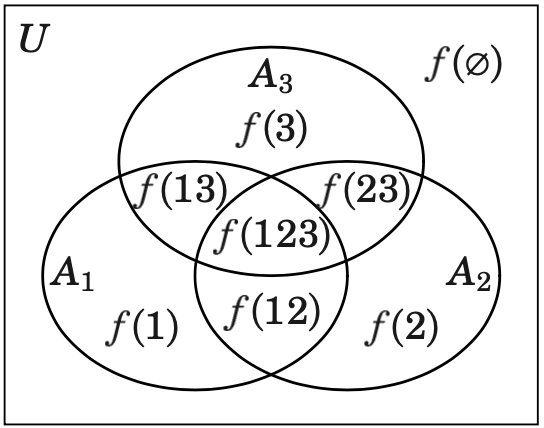
\includegraphics[width =
0.65\linewidth]{combinatorics-assets/PIE.png}
\end{figure}
Por convenio, la intersección vacía es $U$.
\begin{theorem}[PIE]
\label{theorem-combi-007}

$$
f(T) =  \sum_{S\supseteq T}(-1)^{|S|-|T|}
\left|\bigcap_{i\in S}A_i \right|
$$

\end{theorem}

Muchas veces se usa el PIE en su forma
complementaria, que es justamente lo que West
denota por $f(\varnothing)$. Una fórmula más
accesible es:
$$
\begin{aligned}
 \left|U-\bigcup_{i = 1}^nA_i \right|& = |U|-
\sum_{i = 1}^n|A_i| +  \ldots +
(-1)^n|A_1\cap \ldots\cap A_n|\\
&=\left|U-\bigcup_{i=1}^nA_i\right|\\
& = |U|- \sum_{i = 1}^n(-1)^{i + 1}
\sum_{\mathcal{A}\in{\{A_1, \ldots,A_n\}
\choose i}} \left|\bigcap \mathcal{A}
\right|\end{aligned}
$$
y en particular, si las intersecciones de los
$A_i$ son todas del mismo tamaño, tenemos la
expresión

$$
 \left|U-\bigcup_{i = 1}^nA_i \right| =
\sum_{k = 0}^n(-1)^k{n \choose k}\alpha_k
$$

donde $\alpha_k$ es el tamaño de las
intersecciones de a $k$, y $\alpha_0 = |U|$.

Una clara aplicación de esta fórmula nos da
una prueba muy directa de un resultado
conocido
\begin{theorem}
\label{%
theorem-stirling-inclusion-exclusion}

$$
S(n,k) =  \frac{1}{k!} \sum_{i = 0}^k(-1)^i{k
\choose i}(k-i)^n
$$

\end{theorem}
\begin{proof}
Recordemos que las particiones de $[n]$ en
$k$ bloques no vacíos se pueden ordenar de
acuerdo a los elementos que tienen, así que
podemos ordenar los bloques en la lista $[k]$
y pensar que las particiones
\textit{ordenadas} $[n]$ en $k$ bloques no
vacíos son funciones suprayectivas de $[n]$
en $[k]$.

Usando PIE, podemos contar estas funciones
calculando el número de funciones de $[n]$ en
$[k]$ menos la unión de las funciones que no
le pegan a $1,2, \ldots k$. Todas las
intersecciones son del mismo tamaño, así que
esta cantidad es $ \sum_{i = 0}^k(-1)^i{k
\choose i}(k-i)^n$. Al ``revolverlas" para
que ya no sean las particiones ordenadas,
dividimos entre $k!$ y listo.
\end{proof}

\section{Enumeración bajo acciones de grupo}
\label{%
section-enumeracion-bajo-acciones-de-grupo}
\begin{theorem}[Lema de conteo de órbitas]
\label{theorem-combi-008}
Dada una acción de un grupo finito $G$ en un
conjunto finito $X$,

$$
|X/G| =  \frac{1}{|G|} \sum_{g\in G}|
\operatorname{Fix} g|
$$

donde $X/G$ es el conjunto de órbitas y $
\operatorname{Fix} g$ es el conjunto de
puntos fijos de $g\in G$.
\end{theorem}
\begin{proof}
Primero notemos que

$$
 \sum_{g\in G}| \operatorname{Fix} g| =
\sum_{x\in X}| \operatorname{Stab} x|
$$

ya que ambos lados cuentan la cantidad de
parejas $(g,x)$ tales que $g$ fija a $x$.

Ahora notemos que, dado $x$, hay tantos
elementos en su órbita como clases laterales
$G/ \operatorname{Stab} x$. En efecto: la
correspondencia $gx\mapsto g
\operatorname{Stab} x$ está bien definida y
es biyectiva. Agregando a esto el teorema de
Lagrange,

$$
|G\cdot x| = [G: \operatorname{Stab} x] =
|G|/| \operatorname{Stab} x|
$$

Invirtiendo este cociente y sumando sobre
$x\in X$, casi terminamos. Sólo falta notar
que como las órbitas son una partición de
$X$,

$$
 \sum_{x\in X} \frac{1}{|G\cdot x|} =
\sum_{G\cdot x\in X/G} \left( \sum_{y\in
G\cdot x} \frac{1}{|G\cdot y|} \right) =
\sum_{G\cdot x\in X/G}1 = |X/G|
$$

\end{proof}
\begin{theorem}[de enumeración de
Pólya-Redfield]
\label{theorem-combi-009}
Sea $X$ un conjunto finito, $G$ un grupo de
permutaciones de $X$ y $Y$ un conjunto finito
de colores. Entonces,

$$
|Y^X/G|=\frac{1}{|G|}\sum_{g\in G}|Y|^{c(g)}
$$

donde:
\begin{itemize}
\item $Y^X$ es el conjunto de coloraciones de
$X$, formalmente el conjunto de funciones
$X\to Y$.
\item Como $G$ actúa en $X$, también actúa en
$Y^X$, así que hay un espacio de órbitas
$Y^X/G$.
\item $c(g)$ es la cantidad de ciclos que
tiene $g$ cuando lo vemos como una
permutación de $X$.
\end{itemize}
\end{theorem}
\begin{remark}
\label{remark-combi-002}
Hay una versión con pesos de este teorema,
que demuestra West. Por ahora no lo
escribimos.
\end{remark}
\begin{definition}
\label{definition-combi-012}
El \emph{índice de ciclo} es un polinomio
Si $m_i(g)$ es el número de ciclos de
longitud $i$ de $g$, entonces

$$
Z_G(x_1,x_2, \ldots) =  \frac{1}{|G|}
\sum_{g\in G}\prod_{i\geq1}x_i^{m_i(g)}.
$$

es decir, cada $x_i$ representa un ciclo de
longitud $i$.
\end{definition}
Por ejemplo, el polinomio

$$
\frac{1}{12}(x^4_1+8x_1x_3+3x^2_2)
$$

Es el índice de ciclos del subgrupo de
rotaciones de las simetrías de un tetraedro
regular, ya que la identidad tiene cuatro
1-ciclos, las rotaciones por el centro de las
caras tienen un 1-ciclo y un 3-ciclo, y las
rotaciones por los puntos medios de las
aristas tienen dos 2-ciclos. Los coeficientes
enteros simplemente nos dicen cuántas hay de
cada una.

\section{Ejercicios de conteo}
\label{section-ejercicios-de-conteo}
Los ejercicios conservan las referencias del
original: W = West, C = Cameron. Las
ediciones y los números de ejercicio están
pendientes de cotejo; los tres últimos llevan
el mismo número en el original.
\medskip\noindent\textbf{Ejercicio W  1.1.1.}
\textbf{Después de tirar $k$ dados, ¿cuál es
la probabilidad de que la suma sea par?}
\begin{proof}[Solución]
La probabilidad es $1/2$. Denotemos por $P_i$
la probabilidad de que la suma sea par cuando
tiramos $i$ dados, y $I_i$ cuando la suma es
impar. Entonces, la probabilidad que
buscamos, $P_k$, se obtiene de dos formas:
cuando al tirar $k-1$ la suma fue par y el
$k$-ésimo también salió par, o bien cuando al
tirar $k-1$ la suma salió impar y el
$k$-ésimo también salió impar. Es decir,

$$
P_k=P_{k-1}\frac{1}{2}+I_{k-1}\frac{1}{2}
$$

Para encontrar $P_{k-1}$, y todos los
anteriores, sucederá exactamente lo mismo:
$$
P_i=P_{i-1}\frac{1}{2}+I_{i-1}\frac{1}{2}
$$

Y de hecho algo análogo pasa con la
probabilidad de que la suma sea impar: tiene
que ser cierto que los $i-1$ dados anteriores
suman par y el $i$-ésimo impar, o bien que
los $i-1$ anteriores sumaron impar y el
$i$-ésimo par. Es decir,
$$
I_i=P_{i-1}\frac{1}{2}+I_{i-1}\frac{1}{2}
$$

Hasta que lleguemos a $P_2$, que se obtiene
sólo si los dos primeros dados sumaron par, o
si los dos sumaron impar, así que $P_2 =
\frac{1}{2} \frac{1}{2} +  \frac{1}{2}
\frac{1}{2} =  \frac{1}{2}$. Y de hecho $I_2
=  \frac{1}{2} \frac{1}{2} +  \frac{1}{2}
\frac{1}{2} =  \frac{1}{2}$. Sustituyendo,
notemos que $P_3 =  \frac{1}{2} \frac{1}{2} +
\frac{1}{2} \frac{1}{2} =  \frac{1}{2}$. Y de
hecho esto sigue sucediendo conforme subimos
el índice hasta llegar a $k$, es decir, $P_k
=  \frac{1}{2} \frac{1}{2} +  \frac{1}{2}
\frac{1}{2} =  \frac{1}{2}$
\end{proof}

\medskip\noindent\textbf{Ejercicio W 1.1.2.}
\textbf{Cuente la cantidad de rectángulos con
área positiva formados por una retícula con
$m$ rectas horizontales y $n$ verticales}
\begin{proof}[Solución]
Cada rectángulo queda determinado por dos
rectas horizontales y dos verticales. Por
tanto hay

$$
{m\choose2}{n\choose2}
$$

rectángulos. Contar sólo las celdas de la
retícula omite los rectángulos mayores.
\end{proof}

\medskip\noindent\textbf{Ejercicio W 1.1.3.}
\textbf{El alfabeto romano tiene 21
consonantes y 5 vocales. ¿Cuántas palabras se
pueden formar con $r$ consonantes y $s$
vocales?}
\begin{proof}[Solución]
Primero escogemos las $r$ posiciones de las
consonantes. En cada una hay $21$ opciones y
en cada posición restante hay $5$ opciones.
La respuesta es

$$
{r+s\choose r}21^r5^s.
$$

\end{proof}

\medskip\noindent\textbf{Ejercicio W 1.1.8.}
\textbf{¿Cuántas manos de 6 cartas se puede
formar con una baraja de 52 cartas de forma
que haya al menos una carta de cada palo?}
\begin{proof}[Solución]
Los tamaños de los cuatro palos en la mano
son $3,1,1,1$ o $2,2,1,1$. Por tanto hay

$$
4{13 \choose3}13^3 + {4 \choose2}{13
\choose2}^2 13^2
$$

manos. Cada mano se cuenta una sola vez.
\end{proof}

\medskip\noindent\textbf{Ejercicio W 1.1.9.}
\textbf{Cuente la cantidad de números enteros
del 0 al 99,999 en los que cada dígito se
repite a lo más dos veces.}
\begin{proof}[Solución]
Usamos la escritura decimal usual, sin ceros
iniciales; el número $0$ se cuenta por
separado. Para palabras de longitud $\ell$
permitiendo ceros iniciales, sea

$$
T_\ell=\sum_{j=0}^{\lfloor\ell/2\rfloor}
{10\choose j}{10-j\choose\ell-2j}
\frac{\ell!}{2^j}.
$$

Aquí $j$ cuenta los dígitos que aparecen dos
veces. Por simetría entre los diez símbolos,
exactamente $9T_\ell/10$ palabras tienen
primer dígito no nulo. La respuesta es

$$
1+\frac9{10}\sum_{\ell=1}^{5}T_\ell=91954.
$$

Si se usaran siempre cinco posiciones,
rellenando con ceros iniciales, la respuesta
sería $T_5 = 91440$; es otra convención.
\end{proof}

\medskip\noindent\textbf{Ejercicio W 1.1.11.}
\textbf{Dada una bolsa con muchísimas canicas
de 4 colores distintos, ¿de cuántas formas
podemos escoger 12 canicas? Cuente las
distintas formas de ordenarlas en una línea.}
\begin{proof}[Solución]
Una elección de 12 canicas de la bolsa
corresponde a un 12-multiconjunto de $[4]$.
Sabemos que hay ${12 + 3 \choose3} = 455$
tales multiconjuntos. Contar las formas de
ordenarlas en una línea es como contar las
funciones de $[12]$ en $[4]$, que son
$4^{12}$ (es un número muy grande).
\end{proof}

\medskip\noindent\textbf{Ejercicio W 2.2.14.}
\textbf{Resuelva las siguientes recurrencias,
dado que $a_0 = a_1 = 1$.}
\begin{itemize}
\item [(a)]$a_n=4a_{n-1}-4a_{n-2}-n+6$
\item[(b)]$a_n=5a_{n-1}-6a_{n-2}+2n-1+2^n$
\end{itemize}
\begin{proof}[Solución]
Para (a), la parte homogénea es $(A + Bn)2^n$
y una solución particular es $2-n$. Las
condiciones iniciales dan

$$
a_n=(n-1)2^n+2-n.
$$

Para (b), la parte homogénea es $A2^n +
B3^n$. Una solución particular es $n +
3-2n2^n$. Las condiciones iniciales dan

$$
a_n=(-7-2n)2^n+5\cdot3^n+n+3.
$$

Sustituyendo se comprueban las recurrencias y
ambas condiciones iniciales.
\end{proof}
\medskip\noindent\textbf{Ejercicio W 4.1.9.}
\textbf{Usa PIE para demostrar que $
\sum(-1)^k{n \choose k}(n-k)^n = n!$.}
\begin{proof}[Solución]
Consideremos $A_i: = \{f:[n]\to[n]:i\notin
\operatorname{img} f\}$. Las permutaciones de
$n$ elementos son las funciones suprayectivas
de $[n]$ en $[n]$ así que

$$
n!=\left|\{f:[n]\to[n]\}-\bigcup A_i\right|
$$

Usando la fórmula de West, esta cantidad es
$$
\begin{aligned}
f(\varnothing)& =
\sum_{S\subseteq[n]}(-1)^{|S|}
\left|\bigcap_{i\in S}A_i \right|\\
&=\sum_{k=0}^n(-1)^k{n\choose k}(n-k)^n
\end{aligned}
$$
Ya que cada subcolección de $k$ de los
conjuntos $A_i$ tiene intersección de tamaño
$(n-k)^n$, ya que son las palabras de
longitud $n$ en $n-k$ símbolos, y hay ${n
\choose k}$ elecciones en cada caso. Cuando
$k = 0$ contamos todas las funciones de $[n]$
en $[n]$, de las que hay $n^n$.
\end{proof}

\medskip\noindent\textbf{Ejercicio C
3.13.10.}  \textbf{Demuestre las siguientes
identidades:}
\begin{enumerate}
\item ${n \choose k}{k \choose\ell} = {n
\choose\ell}{n-\ell \choose k-\ell}$
\item $ \sum_{i = 0}^k{m \choose i}{n \choose
k-i} = {m + n \choose k}$ donde ${n \choose
k} = 0$ si $k<0$ o $k>n$.
\item $ \sum_{i = 0}^k{n + i \choose i} = {n
+ k + 1 \choose k}$
\item $\sum_{k=1}^nk{n\choose k}=n2^{n-1}$
\item $\sum_{k=0}^{n}(-1)^k{n\choose k}^2=
\begin{cases}
0\qquad(n\equiv1\pmod2)\\
(-1)^m{2m\choose m}\qquad(n=2m)
\end{cases}$
\end{enumerate}
\begin{proof}[Solución]\leavevmode
\begin{enumerate}
\item Ambos lados cuentan los subcomités de
tamaño $\ell$ de los comités de tamaño $k$ de
un grupo de $n$ personas.
\item Ambos lados cuentan los
$k$-subconjuntos de $m + n$.
\item Pendiente en las notas originales.
\item Ambos lados cuentan la cantidad de
parejas $(m,M)$ con $m\in[n]$ y $M\subseteq
[n]$ tales que $m\in M$.
\item Pendiente: demostrar la identidad
alternada del inciso (e).
\end{enumerate}
\end{proof}
\medskip\noindent\textbf{Ejercicio C
3.13.10.}  \textbf{¿Cuántas palabras se
pueden formar con las letras en la palabra
STATE?}
\begin{proof}[Solución]
Tenemos cinco símbolos, así que la cantidad
de permutaciones en total es de $5! = 120$.
Sin embargo, cada intercambio de la letra T
nos lleva a la misma palabra. Para tomar esto
en cuenta consideremos el siguiente
razonamiento. Renombrando los símbolos como
$\mathrm{T}_1$ y $\mathrm{T}_2$, la cantidad
de permutaciones se puede dividir en dos
bloques: los que tienen primero a
$\mathrm{T}_1$ y los que tienen primero a
$\mathrm{T}_2$. Así, la cantidad total de
permutaciones salvo permutaciones de las Ts
es $5!/2 = 60$.
\end{proof}
\medskip\noindent\textbf{Ejercicio C
3.13.10.}  \textbf{¿Cuántas palabras se
pueden formar con $n$ letras si $m$ de ellas
son iguales y las restantes son distintas
entre sí y de esa letra?}
\begin{proof}[Solución]
Ahora tenemos $n!$ posibles palabras, y para
cada una, hay $m!$ maneras equivalentes de
acomodar las letras que son iguales. Hay
$n!/m!$ palabras diferentes.
\end{proof}

\section{Conjuntos parcialmente ordenados}
\label{%
section-conjuntos-parcialmente-ordenados}
\begin{definition}
\label{definition-combi-013}
Una \emph{relación} \textit{R} en un conjunto
$X$ es un subconjunto del producto cartesiano
$X\times X$. Escribimos $xRy$ para denotar
$(x,y)\in R$. Un \emph{orden parcial} en $X$
es una relación
\begin{enumerate}
\item[] \emph{reflexiva}: $xRx$ para toda
$x\in X$.
\item[] \emph{antisimétrica}: si  $xRy$ y
$yRx$, entonces $x = y$.
\item[] \emph{transitiva}: si $xRy$ y $yRz$
entonces $xRz$.
\end{enumerate}
Si dos elementos no se pueden comparar
mediante un orden parcial, escribimos $x||y$.
\end{definition}
\begin{definition}[Conceptos básicos]
\label{definition-combi-014}\leavevmode
\begin{itemize}
\item   Una \emph{cadena} es un conjunto
linealmente ordenado. El \emph{alto} de un
orden parcial es el tamaño de la cadena más
grande.
\item Una \emph{anticadena} es un conjunto
donde no hay dos elementos comparables. El
\emph{ancho} de un orden parcial es el tamaño
de la anticadena más grande.
\item Un elemento en un conjunto parcialmente
ordenado es \emph{maximal} (\emph{minimal})
si no hay elementos mayores (menores) que él.
\item Un elemento es el \emph{máximo}
(\emph{mínimo}) si es mayor (menor) o igual
que todos los demás. El máximo y el mínimio
son únicos.
\item Dos conjuntos parcialmente ordenados
son \emph{isomorfos} si existe una biyección
entre ellos que preserva y refleja el orden.
\item El \emph{producto} de dos COPOS está
construido en el producto cartesiano de los
conjuntos y la relación de orden está dada
entrada a entrada.
\end{itemize}
\end{definition}
\begin{definition}
\label{definition-combi-015}
Un \emph{diagrama de Hasse} es una gráfica
cuyos puntos son los elementos del COPO y hay
una arista entre dos elementos comparables si
no hay ninguno entre ellos. El elemento mayor
está literalmente arriba (coordenada $y$
mayor). El diagrama determina completamente
el COPO: $u<v$ si y sólo si existe un camino
``vertical" entre $u$ y $v$.
\end{definition}
\begin{definition}[Latices]
\label{definition-combi-016}\leavevmode
\begin{itemize}
\item Una \emph{latiz} es un COPO en el que
cualquier pareja de elementos tiene una
máxima cota inferior (\emph{glb}) y una
mínima cota superiot (\emph{lub}).

Un conjunto totalmente ordenado es una latiz,
ya que cualesquiera dos elementos son
comparables, así que podemos tomar la máxima
cota inferior el menor de ellos, y la mínima
cota superior el mayor de ellos. También el
conjunto potencia es una latiz, donde la glb
es la intersección y la lub la unión.

Usamos la notación $a\wedge b$ para la glb de
$a$ y $b$, y $a\vee b$ para la lub.
\item Una latiz es \emph{distributiva} si
$$
\begin{aligned}
x\vee(y\wedge z)=(x\vee y)\wedge(x\vee z)\\
x\wedge(y\vee z)=(x\wedge y)\vee(x\wedge z)
\end{aligned}
$$
\item Un subconjunto $Y\subseteq P$ de un
COPO es un \emph{down-set} si para
cualesquiera  $y\in Y$ y $z\in P$ tales que
$z\leq y$, se tiene que $z\in Y$. Es decir,
todo lo que está abajo de cualquier elemento
de $Y$ está en $Y$.

La colección de down-sets es una latiz
distributiva, que denotamos $L(P)$. Cualquier
latiz distributiva finita se puede
representar como la $L(P)$ de un COPO en
$[n]$:
\end{itemize}
\end{definition}

\begin{theorem}
\label{theorem-combi-010}
Sea $L$ una latiz distributiva finita.
Entonces hay un único COPO finito, salvo
isomorfismo, tal que $L$ es isomorfo a
$L(P)$.
\end{theorem}
Por ejemplo, el COPO $\mathsf{N}$ tiene la
siguiente latiz distributiva:

\begin{center}
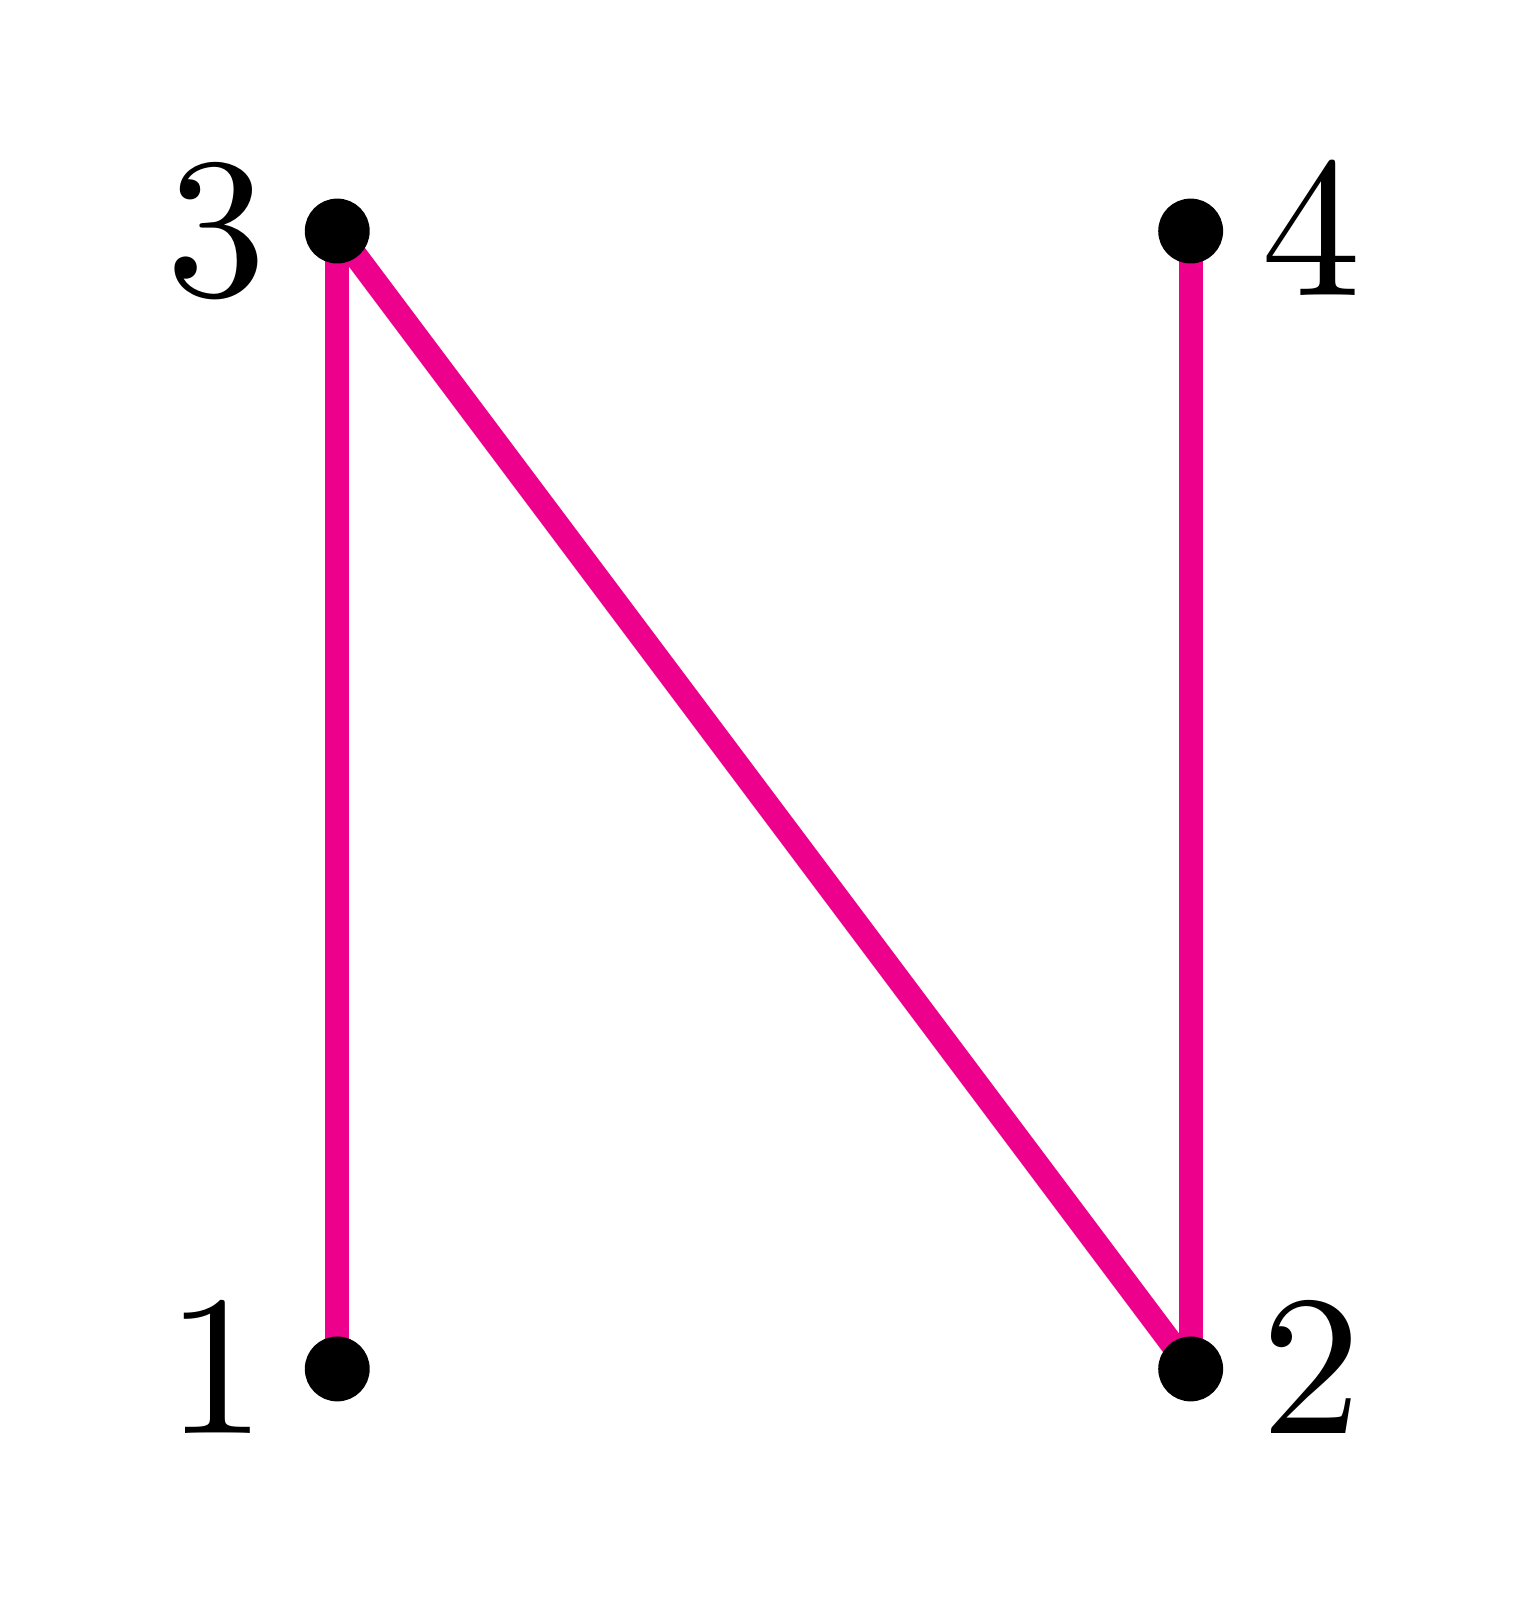
\includegraphics[width =
0.42\linewidth]{
combinatorics-assets/diagram-1.png}
\qquad \qquad
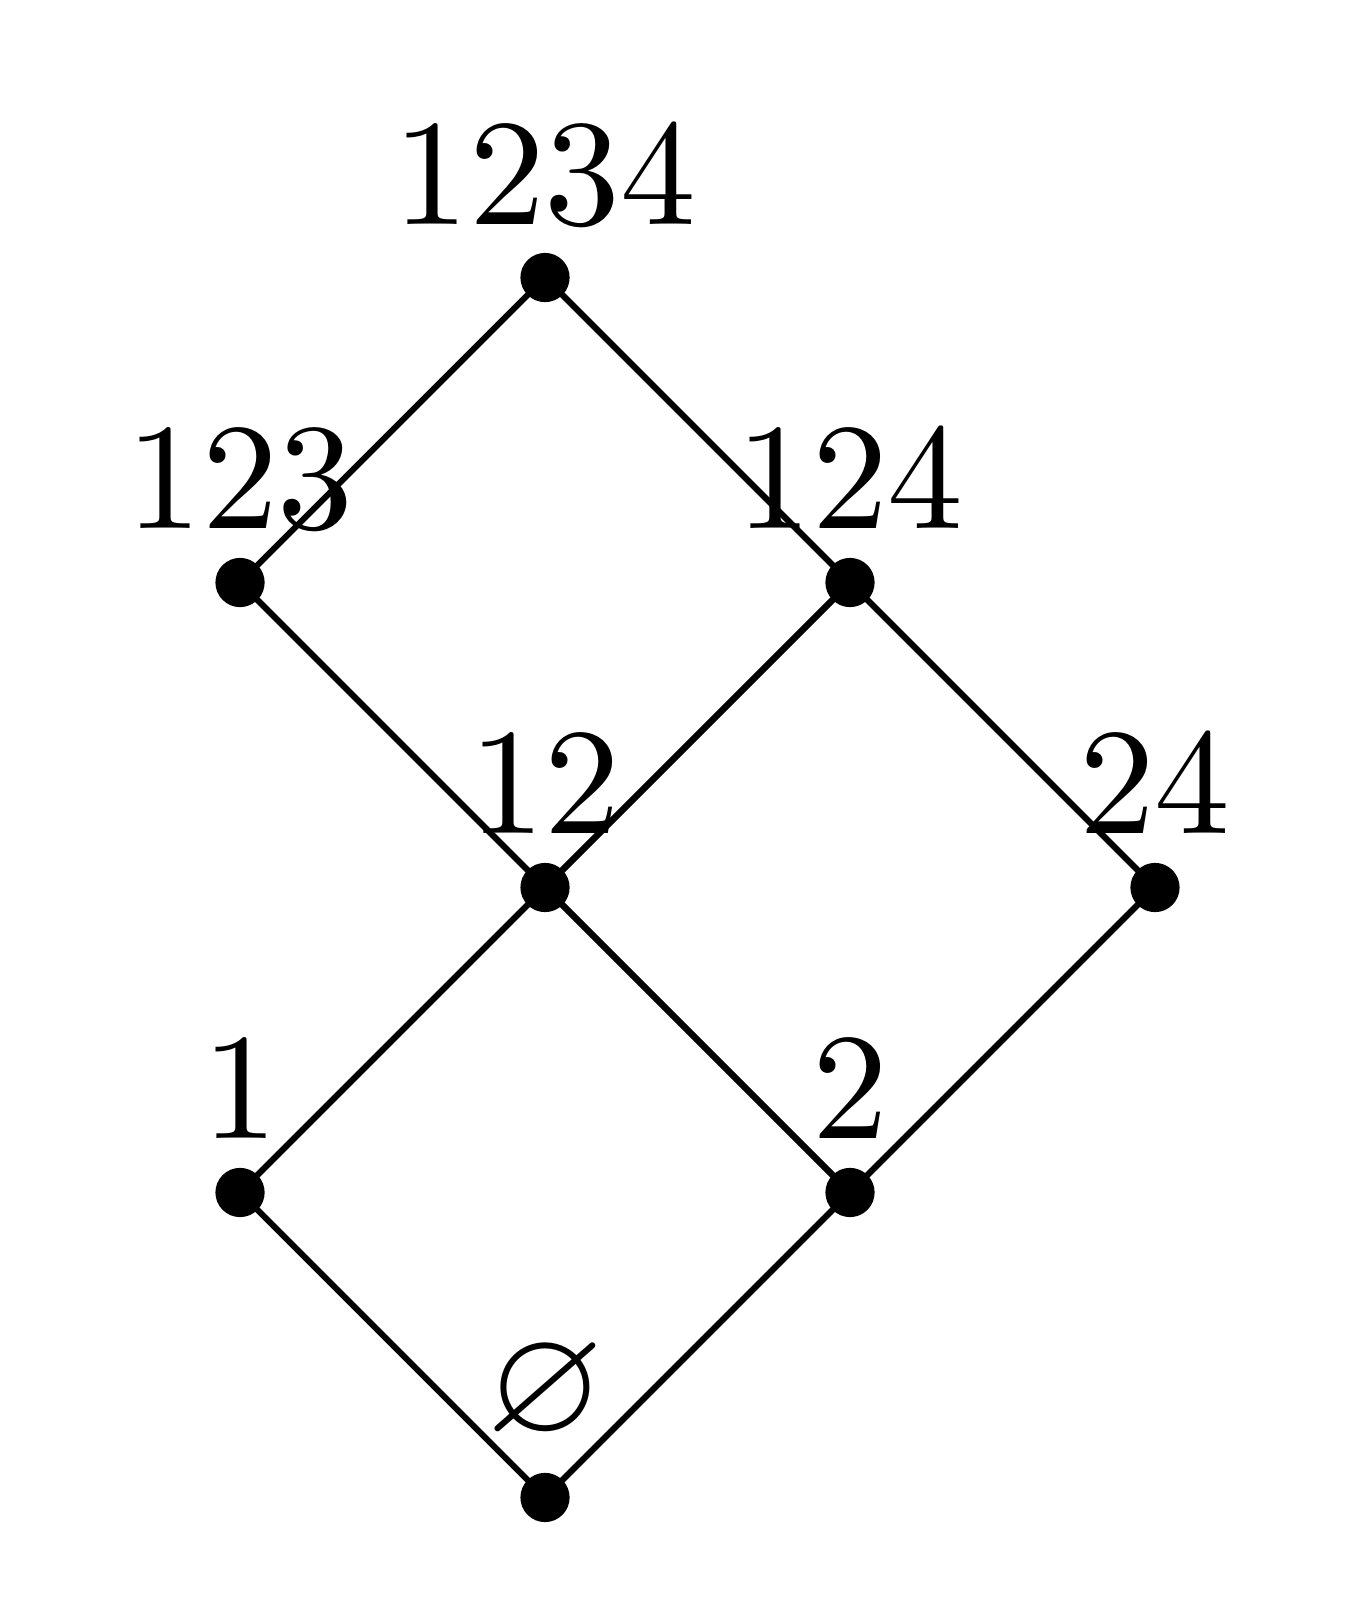
\includegraphics[width =
0.42\linewidth]{
combinatorics-assets/diagram-2.png}
\end{center}

\begin{lemma}
\label{lemma-combi-002}
Cualquier COPO finito no vacío tiene un
elemento maximal.
\end{lemma}
\begin{theorem}[Dilworth, 1950]
\label{theorem-combi-011}
Sea $P$ un orden parcial finito. El tamaño de
la anticadena más grande es igual al mínimo
número de cadenas que forman una partición de
$P$.
\end{theorem}
\begin{proof}
Inducción sobre el tamaño de $P$. La
condición es obvia para un conjunto vacío,
así que podemos tomar un elemento maximal
$a\in P$.

Supongamos que cualquier subconjunto con
menos elementos que $P$ puede ser cubierto
por tantas cadenas y como elementos en la
anticadena más grande. Tomemos
$P\backslash\{a\}$, y supongamos que hay $k$
cadenas $C_1, \ldots,C_k$ que lo cubren y una
anticadena $A_0$ con $k$ elementos. Como
$A_0\cap C_i\neq\varnothing$, podemos escoger
un elemento maximal en $C_i$ que esté en
alguna anticadena de tamaño $k$ para definir
$A: = \{x_1, \ldots,x_k\}$.

Veamos que $A$ es una anticadena. Tomemos dos
elementos $x_i\neq x_j\in A$. Hay una
anticadena $A_i$ de tamaño $k$ en la que está
$x_i$, y de hecho $A_i\cap
C_j\neq\varnothing$ ya que las $C$'s cubren
todo el copo. Escojamos $y\in A_i\cap C_j$.
Como $y$ está en la cadena cuyo elemento
maximal es $x_j$, tenemos que $y\leq x_j$.
Pero $y$ está en una anticadena donde está
$x_i$, así que no es posible que $y\leq x_i$
ni que $x_i\leq y$. Luego, si $x_j\leq x_i$
se obtiene una contradicción. Intercambiando
los roles de $i$ y $j$ se obtiene el otro
lado.

Ahora volvamos a $P$. Primero supongamos que
$a\geq x_i$ para alguna $i$ y definamos $K: =
\{a\}\cup\{x\in C_i:x\leq x_i\}$. ¿Qué tan
grande puede ser una anticadena en
$P\backslash K$? Como las $C$'s son una
partición de $P\backslash\{a\}$, cualquier
anticadena de tamaño máximo en
$P\backslash\{a\}$ debe contener algún
elemento de $C_i$. Pero $x_i$ es el elemento
maximal que está en alguna anticadena de
$P\backslash\{a\}$, y ya no está en
$P\backslash K$. Así que $P\backslash K$ no
puede tener una anticadena con $k$ elementos.

Como $A\backslash\{x_i\}$ es una anticadena
de tamaño $k-1$ en $P\backslash K$, por
hipótesis inductiva hay $k-1$ cadenas
disjuntas que lo cubren. Luego, la anticadena
de mayor tamaño en $P$ tiene tantos elementos
como la partición de $C$'s con la $K$.

Por último, si $x_i\not\leq a$ para toda $i$,
entonces $A\cup \{a\}$ es una anticadena,
pues, al ser maximal tampoco podría ser que
$a\leq x_i$. Luego, la partición $\{a\},C_1,
\ldots,C_k$ consiste de $k + 1$ cadenas, el
tamaño de la anticadena más grande en $P$.
\end{proof}
De hecho, el teorema de
Hall (\ref{chap-hall}) se puede deducir de
éste:
\begin{corollary}[Teorema de
Hall]\label{theorem-hall}
Si $X$ es un conjunto finito y $A_1,
\ldots,A_n$ son subconjuntos de $X$ tales que
$ \left|\bigcup_{i\in J}A_i \right|\geq|J|$
para cualquier $J\subseteq[n]$, entonces
existe un sistema de representantes distintos
de los $A_i$.
\end{corollary}
\begin{proof}
Consideremos el orden parcial en el conjunto
de los elementos de $X$ y los símbolos $y_1,
\ldots,y_n$ con la relación $x\leq y_i$ si y
sólo si $x\in A_i$. Tanto $Y = \{y_i\}$ como
$X$ son anticadenas. De hecho, la anticadena
más grande es $X$. Para verlo, supongamos que
$S$ es otra anticadena y consideremos $J =
\{i\in[n]:y_i\in S\}$. Entonces ningún
elemento en los $A_j$ para $j\in J$ puede
estar en $S$. Luego,

$$
|S|\leq|J| + |X|- \left|\bigcup_{i\in J}A_i
\right|\leq|X|
$$

por la condición de Hall.

Así que hay una descomposición del COPO en
tantas cadenas como elementos en $X$.
Entonces, para cada $y_i$ hay al menos una
cadena $x_i<y_i$ que lo contiene. Como hay
tantas cadenas como elementos en $X$, no
puede haber dos $y_i$ que contengan al mismo
elemento, ya que cada $x$ debe estar en una
única cadena.
\end{proof}
Y de hecho la otra implicación también es
cierta: los dos teoremas son equivalentes.
Aquí sólo probaremos este caso particular:
\begin{exercise}
\label{exercise-combi-002}
Hall implica Dilworth para COPOS de dos
niveles.
\begin{itemize}
\item Un COPO de dos niveles está formado por
dos anticadenas $U$ and $L$ de forma que las
únicas relaciones son de la forma $\ell\leq
u$ para $u\in U$ y $\ell\in L$.
\item Conviene usar esta variante de Hall: si
$A_1, \ldots,A_n$ son subconjuntos de un
conjunto finito $X$ tales que $
\left|\bigcup_{i\in J}A_i \right|\geq|J|-r$
para un número $r$ y cualquier $J\subseteq
[n]$, entonces hay una subfamilia de tamaño
$n-r$ con un sistema de prepresentantes
distintos.
\end{itemize}
\end{exercise}

\begin{definition}[Extensiones]
\label{definition-combi-017}\leavevmode
\begin{itemize}
\item Una \emph{extensión} de un COPO $P$ es
un orden parcial en los elementos de $P$ que
contiene todas las relaciones de $P$. Es
decir, si $\leq$ y $\preccurlyeq$ son órdenes
parciales en un conjunto $P$, $\preccurlyeq$
es una extensión de $\leq$ si $a\leq
b\implies a\preccurlyeq b$.

\item Una \emph{extensión lineal} es una
extensión que es una cadena.

\item La \emph{intersección} de dos órdenes
parciales es la colección de relaciones que
aparecen en ambos, es decir, la intersección
de $(P,\leq)$ y $(P,\preccurlyeq)$ es el
orden $(P,\leq^*)$ dado por $a\leq^*b$ si y
sólo si $a\leq b$ y $a\preccurlyeq b$.
\end{itemize}
\end{definition}

\begin{theorem}
\label{theorem-combi-012}
Un COPO finito es la intersección de todas
sus extensiones lineales.
\end{theorem}

\begin{theorem}
\label{theorem-combi-013}
Todo COPO finito tiene una extensión lineal.
Más aún, si $a$ y $b$ no son comparables, hay
una extensión lineal $\preccurlyeq_1$ tal que
$a\preccurlyeq_1 b$ y otra $\preccurlyeq_2$
tal que $b\preccurlyeq_2 a$.
\end{theorem}

\begin{definition}[Orden y dimensión]
\label{definition-combi-018}\leavevmode
\begin{itemize}
\item Un \emph{realizador} de un COPO $P$ es
un es una colección de órdenes lineales cuya
intersección es $P$.
\item La \emph{dimensión} de un COPO $P$ es
el mínimo número de órdenes lineales cuya
intersección es $P$.
\end{itemize}
\end{definition}
Aprovechemos para citar algo de Matousek:
\begin{definition}
\label{definition-combi-019}
Un \emph{encaje} de COPOS es una función
inyectiva que preserva y refleja el orden.
\end{definition}
\begin{theorem}
\label{theorem-combi-014}
Cualquier COPO $(P,\leq)$ se puede encajar en
$(2^X,\subseteq)$.
\end{theorem}

\section{Teoría extremal de conjuntos}
\label{%
section-teoria-extremal-de-conjuntos}
En este capítulo consideraremos familias de
subconjuntos de algún conjunto con ciertas
propiedades, y trataremos de acotar su
tamaño.

\section{Erdős-Ko-Radó}
\label{section-erdos-ko-rado}
Un ejemplo de una familia de $r$-subconjuntos
de un $n$-conjunto que se intersectan dos a
dos se obtiene al tomar un punto del conjunto
total y considerar todos los $r$-subconjuntos
que lo contienen. Sólo cuando $n\geq2r$ el
problema es no trivial, y de hecho en este
caso nuestro ejemplo es la cota mayor para el
tamaño de una subfamilia intersectante. Si $n
= 2r$ hay otros conjuntos que realizan esta
cota, y si $n>2r$, éste es el único.
\begin{theorem}[Erdós-Ko-Rado]
\label{theorem-combi-015}
Supongamos que $n\geq 2r$ y $\mathcal{A}$ es
una familia de $r$-subconjuntos de un
conjunto de $n$ elementos tal que la
intersección de cualesquiera dos de ellos es
no vacía. Entonces

$$
|\mathcal{A}|\leq{n-1\choose r-1}
$$

\end{theorem}
Para ver que cuando $n<2r$ el problema es
trivial, simplemente notamos que cualesquiera
dos elementos se deben intersectar. Luego, la
cantidad de ellos es a lo más ${n \choose
r}>{n-1 \choose r-1}$.
\begin{theorem}[Erdós-Ko-Rado Generalizado]
\label{theorem-combi-016}
Si $n\geq(t + 1)(r-t + 1)$ para un número $t$
tal que la intersección de cualesquiera dos
elementos tiene al menos $t$ elementos,
entonces

$$
|\mathcal{A}|\leq{n-t\choose r-t}
$$

\end{theorem}
\section{Teorema de Sperner}
\label{section-teorema-de-sperner}
\begin{definition}
\label{definition-combi-020}
Una \emph{familia de Sperner} es una familia
de conjuntos tal que ninguno contiene
propiamente a otro. Es justamente una
anticadena.
\end{definition}
Por ejemplo, la colección de todos los
$k$-subconjuntos de $[n]$ es una familia de
Sperner, porque ninguno puede estar
propiamente contenido en el otro ya que esto
implicaría que uno tiene más elementos que el
otro. El valor de $k$ con el que esta familia
puede ser lo más grande posible es $n/2$ si
$n$ es par, y cualquiera de $\lfloor
n/2\rfloor$ o $\lceil n/2\rceil$ si $n$ es
impar. El teorema de Sperner nos dice que
éstos son los tamaños más grandes de las
familias de Sperner en general.

\begin{theorem}[de Sperner]
\label{theorem-combi-017}
Si $\mathcal{F}$ es una familia de Sperner de
subconjuntos de un conjunto con $n$
elementos, entonces

$$
|\mathcal{F}|\leq{n \choose\lfloor
\frac{n}{2}\rfloor}
$$

Y si la igualdad se cumple, entonces
$\mathcal{F}$ consiste de todos los
subconjuntos de tamaño $\lfloor
\frac{n}{2}\rfloor$ o bien de todos los de
tamaño $\lceil \frac{n}{2}\rceil$.
\end{theorem}
\section{De Bruijn-Erdős}
\label{section-de-bruijn-erdos}

Para el enunciado preciso, véase
\cite[Sección 1]{erdos-finite-linear-1983}.

\begin{theorem}[de Bruijn-Erdős]
\label{theorem-combi-018}
Sea $X$ un conjunto de $n\geq3$ puntos y
$\mathcal{F}$ una familia de subconjuntos
propios de $X$, cada uno de tamaño al menos
dos, tal que cada pareja de puntos pertenece
a exactamente un miembro de $\mathcal{F}$.
Entonces

$$
|\mathcal{F}|\geq n
$$

y si $|\mathcal{F}| = n$, entonces se tiene
alguno de los siguientes casos:
\begin{itemize}
\item Hay un punto distinguido, digamos $n$,
tal que $A_i = \{i,n\}$ y $A_n = \{1,
\ldots,n-1\}$, y $1\leq i<n$. En este caso
tenemos un "near pencil".

\begin{center}
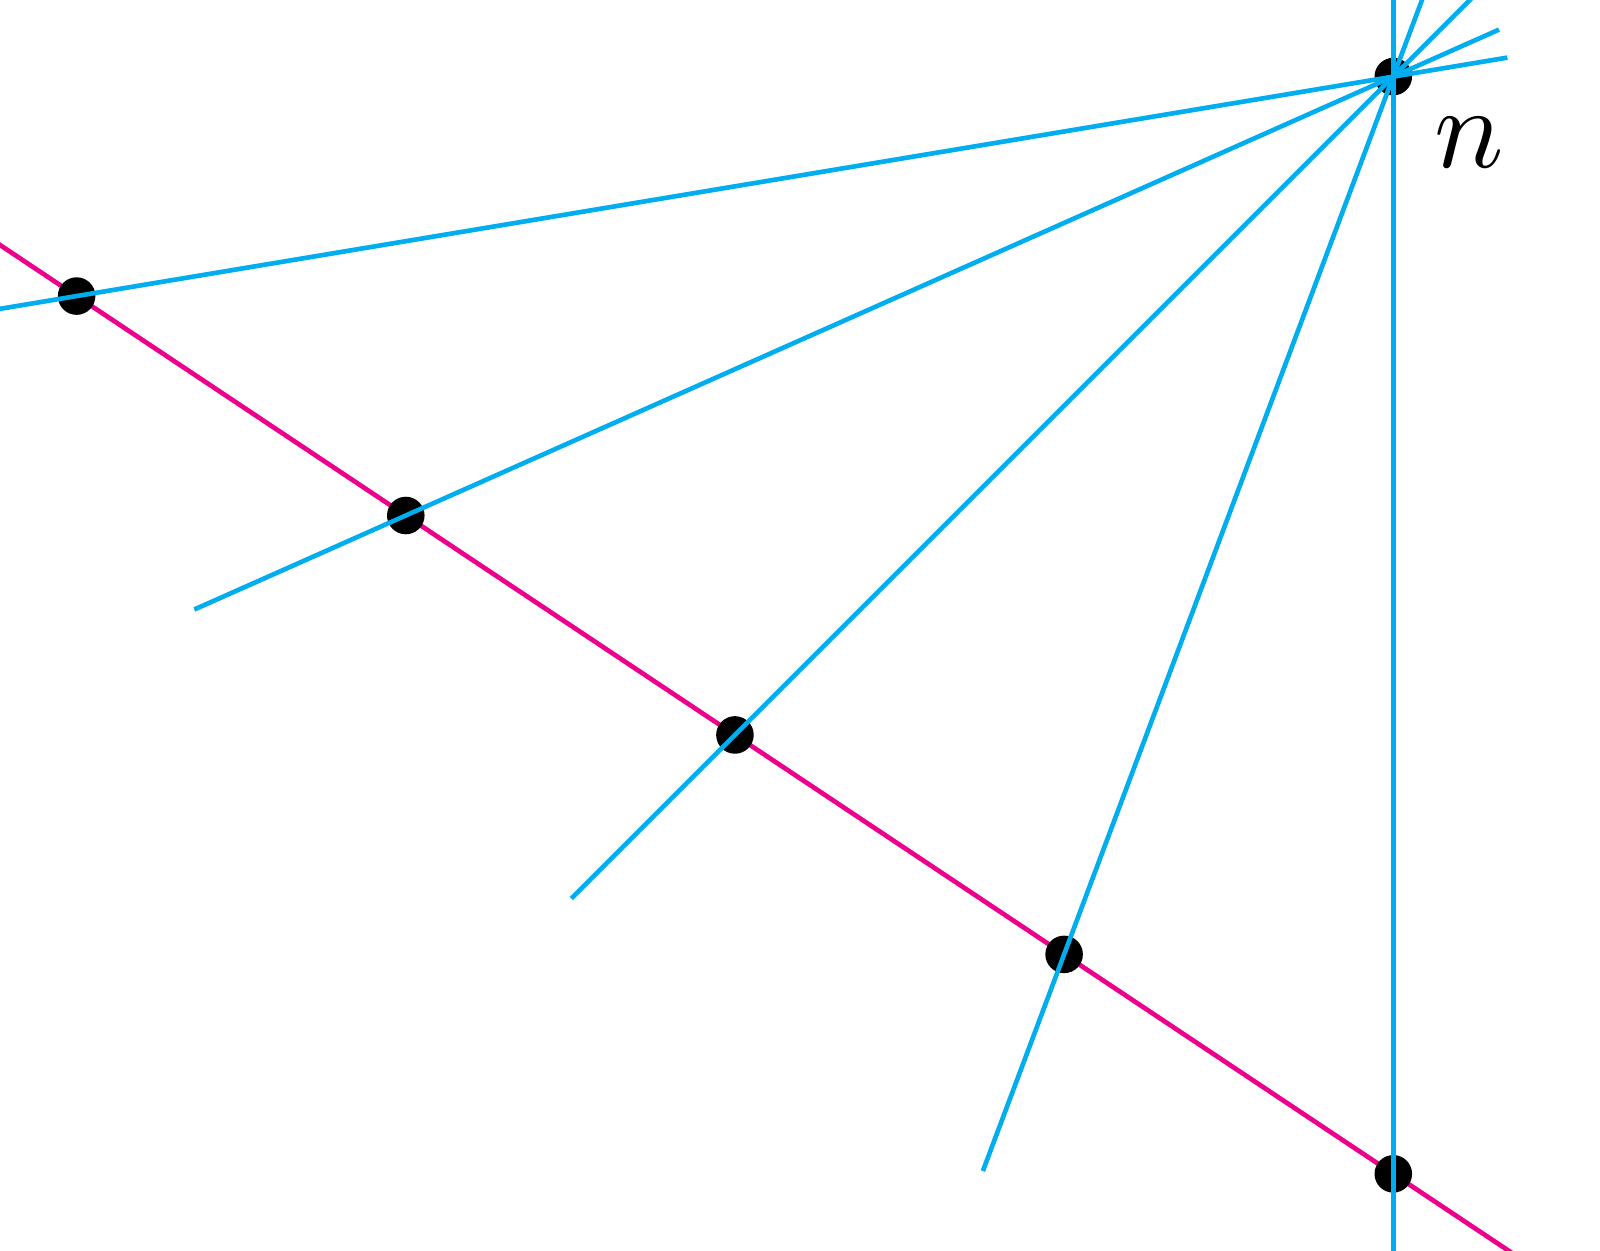
\includegraphics[width =
0.42\linewidth]{
combinatorics-assets/diagram-3.png}
\end{center}

\item $\mathcal{F}$ son las líneas de un
plano proyectivo finito.
\end{itemize}
\end{theorem}
\section{Cuadrados latinos}
\label{section-cuadrados-latinos}
\begin{definition}
\label{definition-combi-021}
Un \emph{cuadrado latino} de \emph{orden} $n$
es una matrix de $n\times n$ tal que cada
entrada está en un único renglón y una única
columna. Dos cuadrados latinos son
\emph{ortogonales} si al sobreponerlos,
ninguna de las $n^2$ entradas es igual. Una
\emph{familia ortogonal} de cuadrados latinos
es una colección de cuadrados latinos
mutualmente ortogonales, y se denota
$\operatorname{MOLS}(n,k)$,
donde $n$ es el orden y $k$ el tamaño
de la familia.
\end{definition}
\begin{lemma}
\label{lemma-combi-003}
Una familia ortogonal de cuadrados latinos de
orden $n$ tiene como máximo $n-1$ elementos.
\end{lemma}
\begin{proof}
Primero renombramos todos los cuadrados de la
familia para que el primer renglón tenga los
símbolos en orden ascendente. Esto hace que
cualquier pareja de cuadrados sobrepuestos
tenga las entradas $(1,1),(2,2),
\ldots,(n,n)$ en el primer renglón.

Ahora tomemos un cuadradito abajo del primer
renglón en cualquier cuadrado latino. Cuando
le ponemos encima otro cuadrado de la
familia, ese cuadradito debe tener una
entrada de la forma $(i,j)$ con $i\neq j$,
porque todas las entradas iguales ya fueron
consideradas en el primer renglón. Luego, hay
uno tipo de entrada distinto para cada
cuadrado en la familia, y hay $n-1$ posibles
entradas.
\end{proof}
\begin{definition}
\label{definition-combi-022}
Una familia de cuadrados latinos de orden $n$
se llama \emph{completa} si tiene $n-1$
elementos.
\end{definition}
\begin{theorem}
\label{theorem-combi-019}
Para cualquier $n$ potencia de primo, hay una
$ \operatorname{MOLS}(n,n-1)$.
\end{theorem}

\section{Teorema de Hall}\label{chap-hall}
\begin{definition}
\label{definition-combi-023}
Sean $A_1, \ldots,A_n$ conjuntos. Un
\emph{sistema de representantes distintos
(SDR)} es una $n$-tupla $(x_1, \ldots,x_n)$
tal que:
\begin{itemize}
\item[(a)] $x_i\in A_i$ para toda $i$.
\item[(b)] $x_i\neq x_j$ para toda $i\neq j$.
\end{itemize}
\end{definition}
Si existe un SDR, para cualquier subconjunto
$J$ de $\{1, \ldots,n\}$, $
\left|\bigcup_{i\in J}A_i \right|\geq|J|$,
pero el converso también es cierto:
El Teorema \ref{theorem-hall}, demostrado
mediante Dilworth, da la suficiencia de esta
condición. La necesidad se sigue porque los
representantes son distintos.
Dados un conjunto de niñas y uno de niños,
dado que cada niño conoce cierto subconjunto
de niñas, es posible casar a cada niño con
una niña que conoce si y sólo si cualquier
$k$-subconjunto de niños corresponde hay al
menos $k$ niñas que alguno de ellos conoce.
Es el teorema de matrimonio de Hall.
\begin{theorem}
\label{theorem-combi-020}
Supongamos que los conjuntos $A_1,
\ldots,A_n$ satisfacen la condición de Hall,
y además $|A_i|\geq r$ para toda $i$ y algún
número $r$. Entonces, la cantidad de SDRs que
hay es al menos:

$$
\begin{cases}
r!\qquad&r\leq n\\
r(r-1)\ldots(r-n+1)=\frac{r!}{(r-n)!}&r>n
\end{cases}
$$

\end{theorem}
\begin{theorem}
\label{theorem-combi-021}
Supongamos que $A_1, \ldots,A_n$ son
subconjuntos de $\{1, \ldots,n\}$ y $r$ es un
entero positivo tal que
\begin{itemize}
\item[(a)] $|A_i|=r$ para toda $i$.
\item[(b)] Cualquier elemento de $\{1,
\ldots,n\}$ está contenido en exactamente $r$
de los subconjuntos.
\end{itemize}
Entonces, la familia satisface la condición
de Hall, así que tiene un SDR.
\end{theorem}
\begin{corollary}
\label{corollary-combi-002}
Esta familia tiene al menos $r!$ SDRs.
\end{corollary}
Estos resultados se usan para completar
cuadrados latinos. Ver Proofs from the Book.
\section{Diseños de bloques}
\label{section-disenos-de-bloques}
\begin{definition}
\label{definition-combi-024}
Un $t$-$(v,k,\lambda)$\emph{-diseño de
bloques} es una colección $\mathcal{B}$ de
subconjuntos de algún conjunto $V$ tales que:
\begin{itemize}
\item $V$ tiene $v$ elementos.
\item Cada bloque en $\mathcal{B}$ tiene $k$
elementos.
\item Cualquier familia de $t$ elementos en
$V$ está en exactamente $\lambda$ bloques en
común.
\end{itemize}
\end{definition}
\begin{definition}
\label{definition-combi-025}
La \emph{matriz de incidencia} de un diseño
de bloques es una matriz de ceros y unos
cuyos renglones son los elementos de $V$ y
las columnas son los bloques que indica si un
elemento está en ese bloque.
\end{definition}
\begin{proposition}
\label{proposition-combi-002}
Un $(v,k,\lambda)$-diseño de bloques que
tiene $b$ bloques y cualquier elemento de $V$
aparece en $r$ bloques satisface que:
\begin{enumerate}
\item $vr=kb$
\item $\lambda(v-1)=r(k-1)$
\end{enumerate}
\end{proposition}
\begin{proof}\leavevmode
\begin{enumerate}
\item Ambos lados de la igualdad son formas
de contar la cantidad de 1's en la matriz de
incidencia.
\item Dado $x\in V$, ambos lados de la
igualdad son formas de contar la cantidad de
pares $(y,B)$ con $y\neq x$ y $x,y\in B$.
\end{enumerate}
\end{proof}
Hay una generalización de la proposición
anterior para diseños de bloques con
$t\neq2$:
\begin{proposition}
\label{proposition-combi-003}
Si un $t$-$(v,k,\lambda)$-diseño de bloques
existe, entonces el siguiente número es un
entero para $0\leq s\leq t$:

$$
\lambda \frac{{v-s \choose t-s}}{{k-s \choose
t-s}} = \lambda \frac{(v-s)(v-s-1) \ldots(v-t
+ 1)}{(k-s)(k-s-1) \ldots(k-t + 1)}
$$

\end{proposition}
Los casos $s=0$ y $s=1$ dan el número de
bloques y el número de bloques por punto,
respectivamente.
En esta sección, $(v,k,\lambda)$ significa
$2$-$(v,k,\lambda)$; suponemos $2\leq k<v$ y
$\lambda>0$ para la desigualdad de Fisher.
\begin{theorem}[Desigualdad de Fisher]
\label{theorem-combi-022}
Si $k<v$, entonces $b\geq v$.
\end{theorem}
\begin{proof}
Consideramos la matriz de incidencia $A$,
cuya entrada $i,j$ es

$$
a_{ij}=\begin{cases}
1 & x_i\in B_j\\
0 & x_i\notin B_j
\end{cases}
$$

Luego, la matriz $AA^T$ tiene entrada $i,j$

$$
m_{ij}=\sum_{k=1}^ba_{ik}a_{jk}
$$

que representa la cantidad de bloques en
donde están al mismo tiempo los elementos
$x_i$ y $x_j$. Por definición, esta cantidad
es

$$
m_{ij}=\begin{cases}
\lambda & i\neq j\\
r & i=j
\end{cases}
$$

Esta matriz es $(r-\lambda)I + \lambda J$,
donde $J$ tiene todas sus entradas iguales a
uno. Como $r = \lambda(v-1)/(k-1)>\lambda$,
sus valores propios $r-\lambda$ y $r +
(v-1)\lambda$ son positivos. Tiene
determinante distinto de cero, por lo que al
ser una matriz de $v\times v$ tiene rango, es
decir, la dimensión del espacio lineal
generado por las columnas, igual a $v$.

Para concluir notemos que si $b<v$, cada
matriz tiene como mucho $b$ columnas o
renglones, respectivamente, así que el rango
de $A$ y de $A^T$ sería menor estricto que
$v$. Como el rango del producto es menor o
igual al mínimo de los rangos de los
factores, $ \operatorname{ran} M<v$, que no
es posible.
\end{proof}
Este teorema sirve para descartar la
existencia de ciertos diseños de bloques,
como por ejemplo $2-(16,6,1)$.

En fin,
\begin{definition}
\label{definition-combi-026}
Un diesño de bloques es \emph{simétrico} si
$v = b$, que implica que $r = k$.
\end{definition}
Va a resultar que podremos voltear el diseño.
Ahí va:
\begin{proposition}
\label{proposition-combi-004}
En un diseño de bloques simétrico, no sólo
cada pareja de elementos está en $\lambda$
bloques, sino que cada pareja de bloques se
intersecta en $\lambda$ elementos.
\end{proposition}
\begin{proof}
Tomemos un bloque arbitrario $B$ y veamos que
su intersección con todos los demás es de
tamaño $\lambda$. Denotemos por $x_1,
\ldots,x_{v-1}$ el tamaño de la intersección
de $B$ con el $i$-ésimo bloque. Mostraremos
que $ \sum(x_i-\lambda)^2 = 0$.

Cada elemento de $B$ está en $k-1$ bloques
además de $B$. Así que hay $k(k-1)$ elementos
en la intersección de $B$ con algún otro
bloque, es decir, $ \sum x_i = k(k-1) =
\lambda(v-1)$ aplicando nuestra proposición.

Análogamente, cada pareja en $B$ está en
$\lambda -1$ bloques además de $B$, así que
hay ${k \choose 2}(\lambda-1)$ parejas en la
intersección de $B$ con otro bloque, es
decir, $ \sum{x_i \choose 2} = {k \choose
2}(\lambda-1)$. Podemos reescribir esto como
$ \sum x_i(x_i-1) = k(k-1)(\lambda-1) =  \sum
x_i^2-x_i = \lambda(v-1)(\lambda-1)$.

Sumando las dos igualdades obtenemos que $
\sum x_i^2 = \lambda(v-1) +
\lambda(v-1)(\lambda-1) = \lambda^2(v-1)$. Y
luego:
$$
\begin{aligned}
 \sum(x_i-\lambda)^2& =  \sum x_i^2-2
\sum\lambda x_i +  \sum \lambda^2\\
& = \lambda^2(v-1)-2\lambda(\lambda(v-1) +
(v-1)\lambda^2 = 0
\end{aligned}
$$
\end{proof}
\begin{remark}
\label{proposition-combi-005}
La condición aritmética para $v$ par es el
primer caso del siguiente teorema.
\end{remark}
\begin{theorem}[Bruck-Ryser-Chowla]
\label{theorem-combi-023}
Si existe un $(v,k,\lambda)$-diseño de
bloques simétrico, entonces
\begin{enumerate}
\item[\textit{(a)}] Si $v$ es par,
$k-\lambda$ es un cuadrado.
\item[\textit{(b)}] Si $v$ es impar, entonces

$$
z^2=(k-\lambda)x^2+(-1)^{(v-1)/2}\lambda y^2
$$

tiene una solución entera no cero en $x,y,z$.
\end{enumerate}
\end{theorem}
\section{Matrices de Hadamard}
\label{section-matrices-de-hadamard}
¿Qué tan grande puede ser el determinante de
una martiz cuyas entradas están acotdadas?
\begin{theorem}[de Hadamard]
\label{theorem-combi-024}
Sea $A$ una matriz de $n\times n$ de números
reales tal que $|a_{ij}|\leq1$ para toda
$i,j$. Entonces, $|\det A|\leq n^{n/2}$, y la
igualdad se satisface si y sólo si $a_{ij} =
\pm1$ y $AA^T = nI$.
\end{theorem}
\begin{proof}
El valor absoluto del determinante es el
volumen del
paralelepípedo $n$-dimensional cuyos lados
son los renglones de $A$. Este volumen es
menor o igual al producto del tamaño de los
lados, que es $\sqrt{ \sum_{j = 1}^n
a_{ij}^2}$ para el $i$-ésimo renglón. Este
número es menor o igual que $\sqrt{n}$, así
que se sigue la desigualdad. La igualdad se
tiene sólo cuando los lados son justo de ese
tamaño, por lo que $|a_{ij}| = 1$, y además
los lados del paralelepípedo son
perpendiculares entre sí, de forma que $
\sum_{k = 1}^na_{ik}a_{jk} = 0$. Esto es
tanto como decir que $AA^T = nI$.
\end{proof}
\begin{definition}
\label{definition-combi-027}
Una matriz que satisface la igualdad en el
teorema anterior es una \emph{matriz de
Hadamard}.
\end{definition}
\begin{proposition}
\label{proposition-combi-006}
Si existe una matriz de Hadamard de orden
$n$, entonces $n = 1$ o $2$, o bien
$n\equiv0\mod4$.
\end{proposition}
\begin{theorem}
\label{theorem-combi-025}
Si $n>4$ es divisible por cuatro, son
equivalentes:
\begin{itemize}
\item Existe una matriz de Hadamard de orden
$n$.
\item Existe un $3$-$(n, \frac{1}{2}n,
\frac{1}{4}n-1)$-diseño de bloques.
\item Existe un $2$-$(n-1, \frac{1}{2}n-1,
\frac{1}{4}n-1)$-diseño de bloques.
\end{itemize}
\end{theorem}
\section{Planos proyectivos finitos}
\label{section-planos-proyectivos-finitos}
\begin{definition}
\label{definition-combi-028}
Un \emph{plano proyectivo finito} es una
pareja $(\mathcal{P},\mathcal{L})$ donde
$\mathcal{P}$ es un conjunto finito de
\textit{puntos} y $\mathcal{L}$ es una
familia de \textit{líneas}, subconjuntos de
$\mathcal{P}$, tales que
\begin{itemize}
\item[\emph{(P0)}] Hay cuatro puntos en
posición general.
\item[\emph{(P1)}] Cualesquiera dos líneas se
intersectan en un único punto.
\item[\emph{(P2)}] Por cualesquiera dos
puntos pasa una única línea.
\end{itemize}
\end{definition}
\begin{lemma}
\label{lemma-combi-004}
Dadas dos líneas, hay un punto que no está en
ellas.
\end{lemma}
\begin{proof}
Cada una de nuestras dos líneas puede
intersectar al conjunto de cuatro puntos, sin
tres colineales, llamémoslo $F$, en a lo más
dos puntos. Si uno de estos cuatro puntos
está fuera de las dos líneas, terminamos, y
si no, nuestras dos líneas están generadas
por dos parejas en $F$, digamos $\ell  =
F^1_\ell\vee F^2_\ell$ y $m = F^1_m\vee
F^2_m$. Ahora tomemos las parejas
$F^1_\ell\vee F^1_m: = a$ y $F^2_\ell\vee
F^2_m: = b$. Si el punto $P = a\wedge b$ está
en $\ell$, entonces $F^1_\ell$, $F^2_\ell$ y
$F^1_m$ estarían en la misma línea, pero esto
no es posible. Lo mismo sucede para $m$.
\end{proof}

\begin{center}
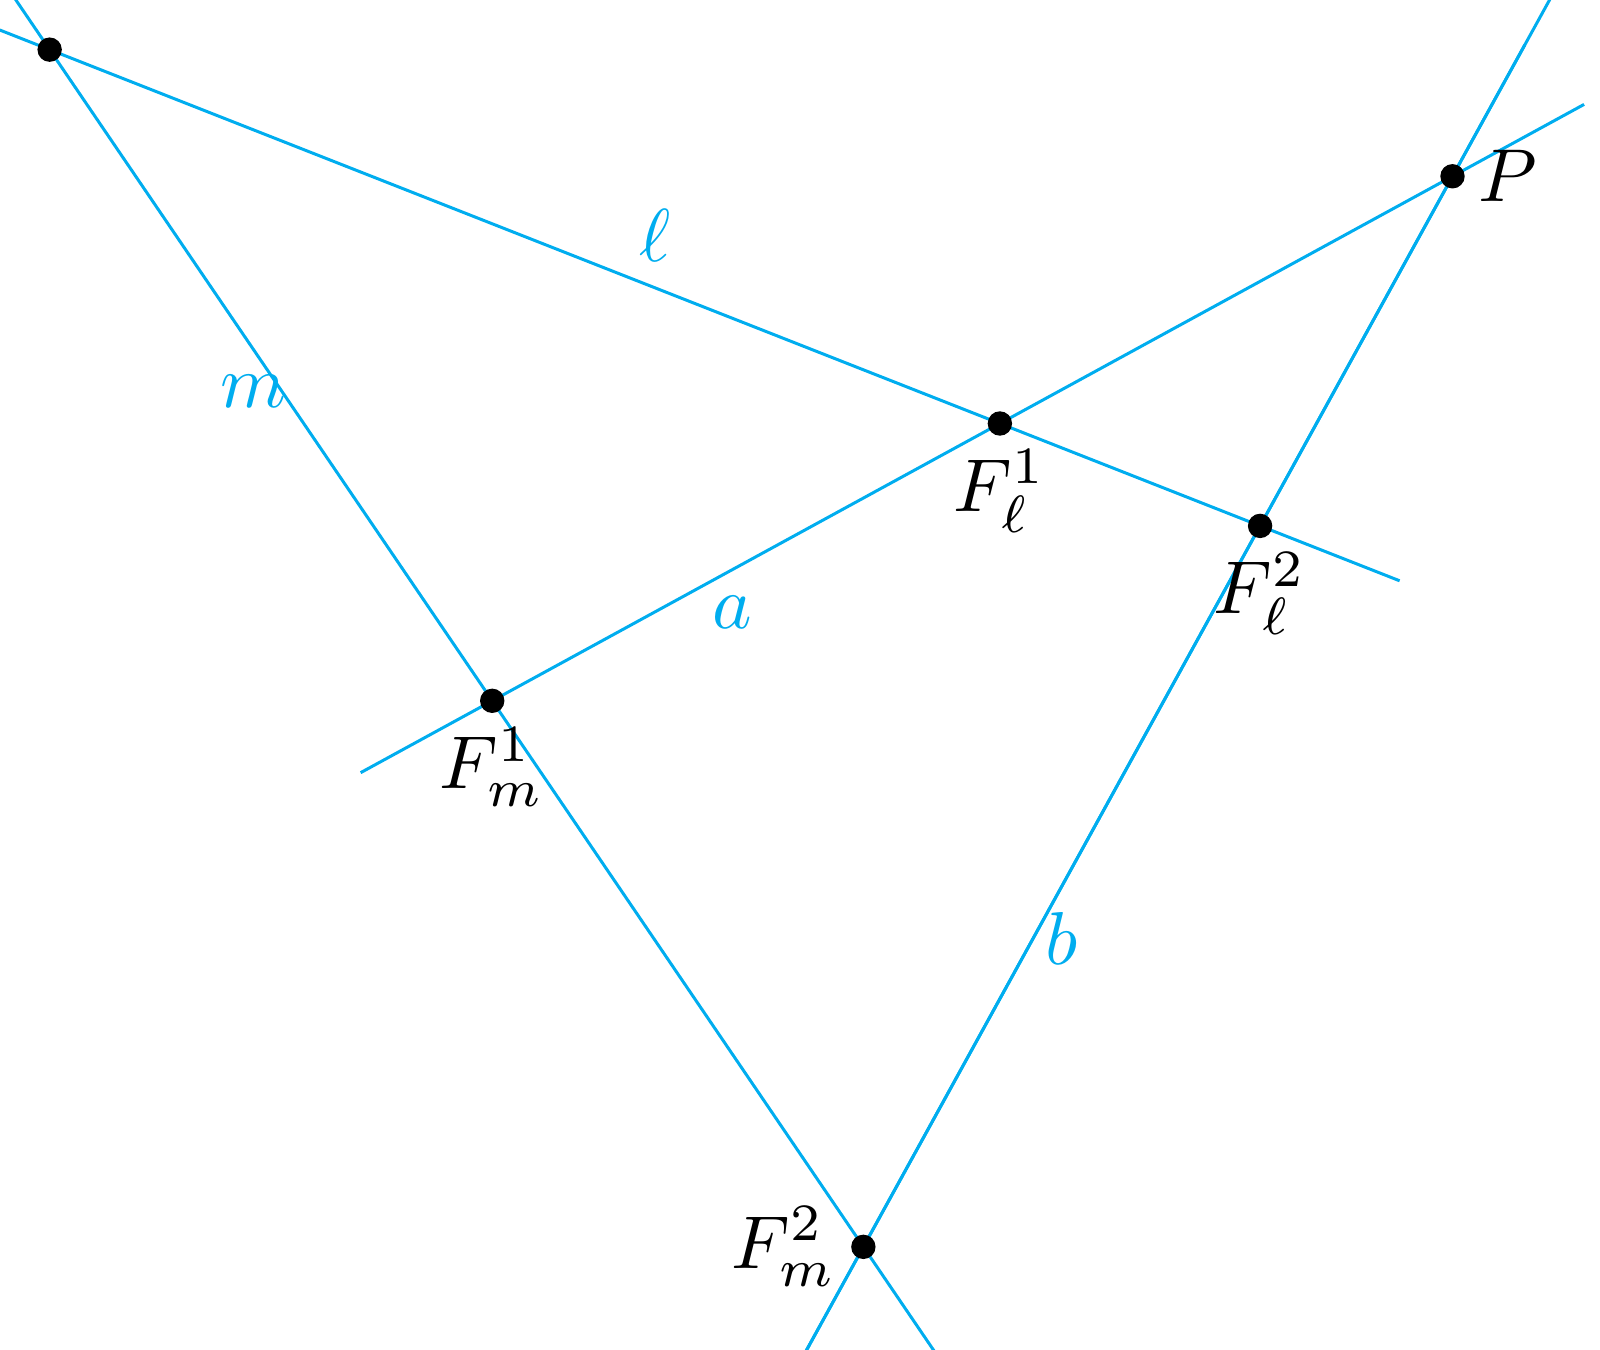
\includegraphics[width =
0.42\linewidth]{
combinatorics-assets/diagram-4.png}
\end{center}

\begin{proposition}
\label{proposition-combi-007}
Todas las líneas tienen la misma cantidad de
puntos.
\end{proposition}
\begin{proof}
Tomemos dos líneas $\ell,m\in\mathcal{L}$ y
un punto $Z$ que no está en ninguna de ellas.
Definamos la proyección que envía un punto
$X\in\ell$ en el punto de intersección de la
recta $XZ$ con $m$.

\begin{center}
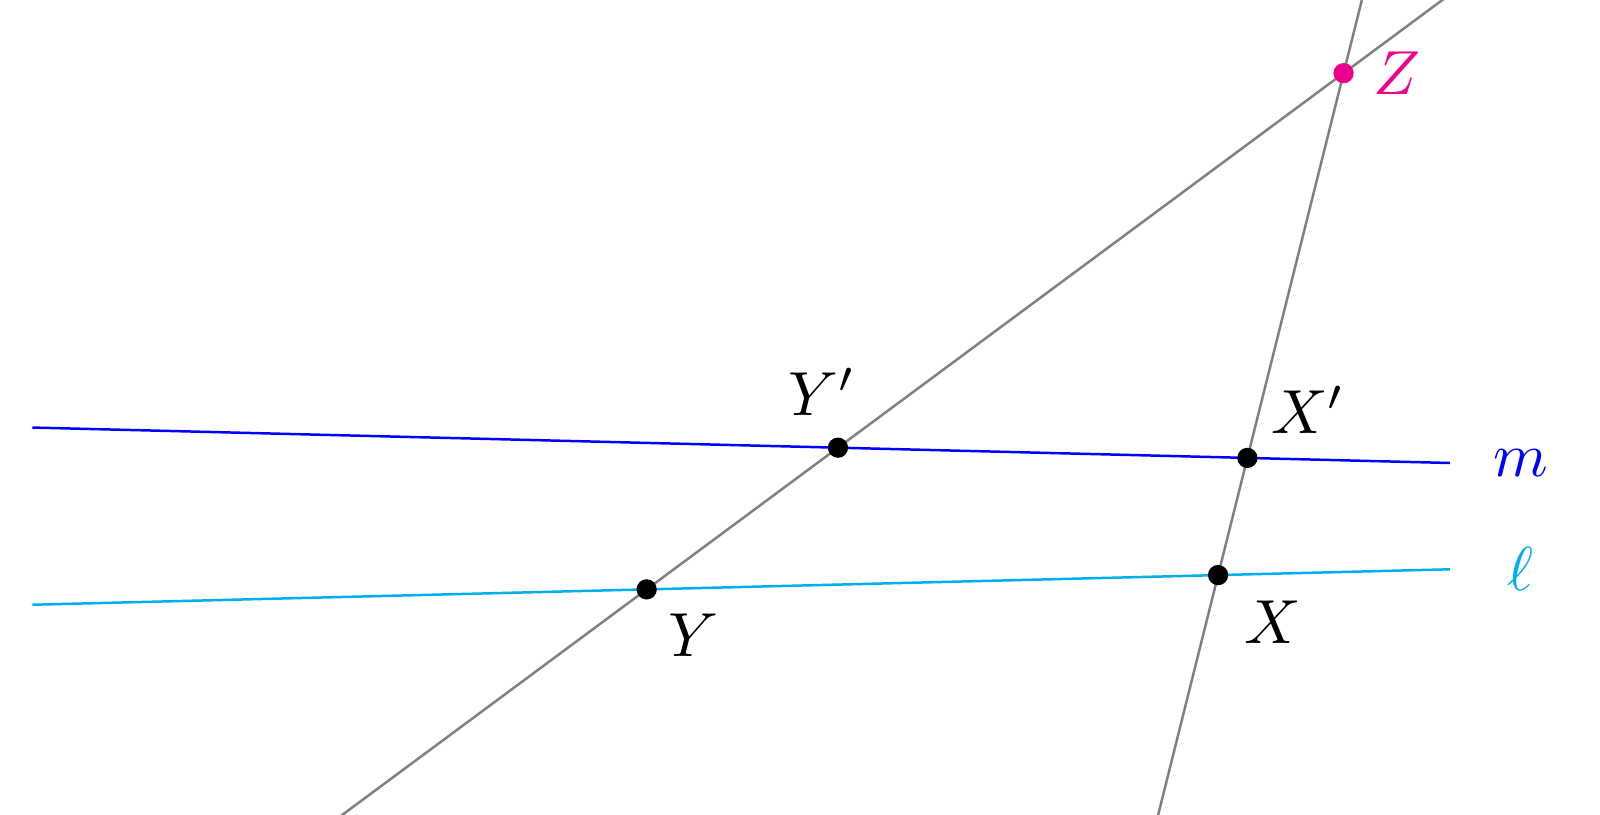
\includegraphics[width =
0.42\linewidth]{
combinatorics-assets/diagram-5.png}
\end{center}

Por (P1), la recta $XZ$ intersecta a $m$ en
un sólo punto, así que la función está bien
definida. Además, es inyectiva, pues si dos
de estas líneas se intersectan en el mismo
punto de $m$, entonces los dos puntos en
$\ell$ de los que provienen, digamos $X$ y
$Y$, de no ser iguales, obligarían a $Z$ a
estar en $\ell$: sólo una línea pasa por
ellos (P2). Intercambiando las dos líneas
se obtiene la función inversa.
\end{proof}
\begin{proposition}
\label{proposition-combi-008}
La cantidad de puntos en una línea es igual a
la cantidad de líneas que pasan por cualquier
punto.
\end{proposition}
\begin{proof}
Pendiente en las notas originales: completar
la demostración mediante la biyección entre
los puntos de una línea y las líneas que
pasan por un punto exterior.
\end{proof}
\begin{definition}
\label{definition-combi-029}
El \emph{orden} del plano proyectivo es el
tamaño de las líneas menos 1.
\end{definition}
\begin{proposition}
\label{proposition-combi-009}
Para $q\geq2$, una familia de conjuntos de
tamaño $q + 1$ es la colección de líneas de
un plano proyectivo de orden $q$ si y sólo si
es un $(q^2 + q + 1,q + 1,1)$-diseño de
bloques.
\end{proposition}
\begin{proof}\leavevmode

($\implies$) Las condiciones \textbf{2} y
\textbf{3} de la definición se satisfacen
trivialmente. Para ver la primera, tomemos
una línea $\ell\in\mathcal{L}$. Para cada uno
de los $q + 1$ puntos en ella pasan $q$
líneas distintas de $\ell$. Esto hace que
haya
exactamente $1 + (q + 1)q = q^2 + q + 1$
líneas.

($\impliedby$) La condición que cualesquiera
dos elementos en $V$ se intersecten en un
sólo bloque nos da la propiedad
\textbf{(P2)}. Usando las fórmulas $vr = kb$
y $\lambda(v-1) = r(k-1)$, obtenemos que $v
= b$ y $r = k$. Es decir, la cantidad de
bloques es igual a la cantidad de puntos, y
cada punto está en tantos bloques como puntos
en cada bloque hay. Estas dos frases implican
que el diseño de bloques es simétrico, luego,
se sigue que cada pareja de bloques se
intersecta en $\lambda = 1$ puntos.
Pendiente: justificar (P0) para completar
esta dirección de la prueba.
\end{proof}
\begin{proposition}
\label{proposition-combi-010}
El \textbf{dual} de un plano proyectivo, la
esctructura que obtenemos al intercambiar los
papeles de la líneas y los puntos preservando
incidencia, también es un plano proyectivo.
\end{proposition}
\begin{theorem}
\label{theorem-combi-026}
Para $q\geq2$, existe un plano proyectivo de
orden $q$ si y sólo si existe una $
\operatorname{MOLS}(q,q-1)$.
\end{theorem}
\section{Ternas de Steiner}
\label{section-ternas-de-steiner}
Después de los planos proyectivos,
consideramos diseños con bloques de tamaño
tres: los sistemas de ternas de Steiner.
\begin{proposition}[Cameron, 8.1.1]
\label{proposition-combi-011}Sea
$\mathcal{B}$ una familia de $m$-subconjuntos
de un $n$-conjunto, con $0\leq l\leq m\leq
n$,
tal que cualquier
$l$-subconjunto está contenida en a lo más un
elemento de $\mathcal{B}$. Entonces

$$
|\mathcal{B}|\leq{n \choose l}\Big/{m \choose
l}
$$

y la igualdad se da cuando cada
$l$-subconjunto está contenido en exactamente
un elemento de $\mathcal{B}$.
\end{proposition}
\begin{proof}
Para la igualdad, se trata de un
$l$-$(n,m,1)$-diseño de bloques. Cualquier
subconjunto de tamaño $l$ está contenido en
exactamente un $m$-bloque. En este caso, los
$l$-subconjuntos del $n$-conjunto están en
correspondencia con los $l$-subconjuntos de
los bloques. Cada bloque tiene ${m \choose
l}$ $l$-subconjuntos.

Si cada $l$ subconjunto está en a lo más un
elemento de $|B|$, puede haber más
$l$-subconjuntos en total que los que les
hacemos corresponder en los bloques.
\end{proof}
\begin{definition}
\label{definition-combi-030}
Una \emph{terna de Steiner} es un
$(v,3,1)$-diseño de bloques, denotado por $
\operatorname{STS}(v)$.
\end{definition}
\begin{theorem}
\label{theorem-combi-027}
Si un $ \operatorname{STS}(v)$ existe,
entonces $v\equiv1,3\pmod6$
\end{theorem}
\begin{proof}
Sustituyendo los valores conocidos en
nuestras fórmulas, obtenemos que

$$
\lambda(v-1) = r(k-1)\iff \frac{v-1}{2} = r
\qquad\implies \qquad vr = kb\approx
\frac{v(v-1)}{6} = b
$$

La primera igualdad quiere decir que $v$ es
impar, así que debe estar en alguna de las
clases equivalencia $\bar{1},\bar{3}$ o
$\bar{5}$ en $\mathbb{Z}_6$. Para ver que no
puede
ser $\bar{5}$, supongamos que $v = 6m + 5$.
Entonces tenemos:

$$
\frac{(6m+5)(6m+4)}{6}=\frac{(6m+5)(3m+2)}{3}
$$

pero ni $6m + 5$ ni $3m + 2$ son múltiplos de
$3$, así que esa fracción no podría ser un
entero, que no es posible.
\end{proof}

\bibliographystyle{alpha}
\bibliography{my}
\end{document}
